%%%%%%%%%%%%%%%%%%%%%%%%%%%%%%%%%%%%%%%%%%%%%%%%%%%%%%%%%%%%%%%%%%%%%%%%%%%%
% AGUJournalTemplate.tex: this template file is for articles formatted with LaTeX
%
% This file includes commands and instructions
% given in the order necessary to produce a final output that will
% satisfy AGU requirements, including customized APA reference formatting.
%
% You may copy this file and give it your
% article name, and enter your text.
%
%
% Step 1: Set the \documentclass
%
%

%% To submit your paper:
\documentclass[draft]{agujournal2019}
\usepackage[utf8]{inputenc}
\usepackage{url} %this package should fix any errors with URLs in refs.
\usepackage{lineno}
\usepackage[inline]{trackchanges} %for better track changes. finalnew option will compile document with changes incorporated.
\usepackage{soul}
\usepackage{amsmath}
\usepackage{listings}
\usepackage{minted}
\linenumbers

\definecolor{mygreen}{rgb}{0,.5,0}
\definecolor{mygray}{rgb}{0.9,0.9,0.9}

\definecolor{psign}{rgb}{0.9  ,0.1,0.1}
\definecolor{pregime}{rgb}{0.9,0.5,0.0}
\definecolor{pregimet}{rgb}{0.6,0.2,0.2}
\definecolor{pexpo}{rgb}{0.1,0.4,0.7}

\newcommand{\op}{\operatorname}

\lstset{ 
  backgroundcolor=\color{mygray},   % choose the background color; you must add \usepackage{color} or \usepackage{xcolor}; should come as last argument
  basicstyle=\ttfamily,        % the size of the fonts that are used for the code
  breakatwhitespace=false,         % sets if automatic breaks should only happen at whitespace
  breaklines=true,                 % sets automatic line breaking
  captionpos=b,                    % sets the caption-position to bottom
  commentstyle=\color{mygreen},    % comment style
  deletekeywords={...},            % if you want to delete keywords from the given language
  escapeinside={\%*}{*)},          % if you want to add LaTeX within your code
  extendedchars=true,              % lets you use non-ASCII characters; for 8-bits encodings only, does not work with UTF-8
  frame=single,	                   % adds a frame around the code
  keepspaces=true,                 % keeps spaces in text, useful for keeping indentation of code (possibly needs columns=flexible)
  keywordstyle=\color{mygreen}\textbf,       % keyword style
  language=Matlab,                 % the language of the code
  morekeywords={julia},            % if you want to add more keywords to the set
  numbers=left,                    % where to put the line-numbers; possible values are (none, left, right)
  numbersep=5pt,                   % how far the line-numbers are from the code
  numberstyle=\tiny\color{gray}, % the style that is used for the line-numbers
  rulecolor=\color{black},         % if not set, the frame-color may be changed on line-breaks within not-black text (e.g. comments (green here))
  showspaces=false,                % show spaces everywhere adding particular underscores; it overrides 'showstringspaces'
  showstringspaces=false,          % underline spaces within strings only
  showtabs=false,                  % show tabs within strings adding particular underscores
  stepnumber=1,                    % the step between two line-numbers. If it's 1, each line will be numbered
  stringstyle=\color{black},     % string literal style
  tabsize=2,	                   % sets default tabsize to 2 spaces
  title=\lstname                   % show the filename of files included with \lstinputlisting; also try caption instead of title
}

\newcommand*\patchAmsMathEnvironmentForLineno[1]{%
  \expandafter\let\csname old#1\expandafter\endcsname\csname #1\endcsname
  \expandafter\let\csname oldend#1\expandafter\endcsname\csname end#1\endcsname
  \renewenvironment{#1}%
     {\linenomath\csname old#1\endcsname}%
     {\csname oldend#1\endcsname\endlinenomath}}% 
\newcommand*\patchBothAmsMathEnvironmentsForLineno[1]{%
  \patchAmsMathEnvironmentForLineno{#1}%
  \patchAmsMathEnvironmentForLineno{#1*}}%
\AtBeginDocument{%
\patchBothAmsMathEnvironmentsForLineno{equation}%
\patchBothAmsMathEnvironmentsForLineno{align}%
\patchBothAmsMathEnvironmentsForLineno{flalign}%
\patchBothAmsMathEnvironmentsForLineno{alignat}%
\patchBothAmsMathEnvironmentsForLineno{gather}%
\patchBothAmsMathEnvironmentsForLineno{multline}%
}

%%%%%%%
% As of 2018 we recommend use of the TrackChanges package to mark revisions.
% The trackchanges package adds five new LaTeX commands:
%
%  \note[editor]{The note}
%  \annote[editor]{Text to annotate}{The note}
%  \add[editor]{Text to add}
%  \remove[editor]{Text to remove}
%  \change[editor]{Text to remove}{Text to add}
%
% complete documentation is here: http://trackchanges.sourceforge.net/
%%%%%%%

\draftfalse

%% Enter journal name below.
%% Choose from this list of Journals:
%
% JGR: Atmospheres
% JGR: Biogeosciences
% JGR: Earth Surface
% JGR: Oceans
% JGR: Planets
% JGR: Solid Earth
% JGR: Space Physics
% Global Biogeochemical Cycles
% Geophysical Research Letters
% Paleoceanography and Paleoclimatology
% Radio Science
% Reviews of Geophysics
% Tectonics
% Space Weather
% Water Resources Research
% Geochemistry, Geophysics, Geosystems
% Journal of Advances in Modeling Earth Systems (JAMES)
% Earth's Future
% Earth and Space Science
% Geohealth
%
% ie, \journalname{Water Resources Research}

\journalname{Journal of Advances in Modeling Earth Systems}


\begin{document}

%% ------------------------------------------------------------------------ %%
%  Title
%
% (A title should be specific, informative, and brief. Use
% abbreviations only if they are defined in the abstract. Titles that
% start with general keywords then specific terms are optimized in
% searches)
%
%% ------------------------------------------------------------------------ %%

% Example: \title{This is a test title}

\title{Weather and climate models in 16bit: Posit, floating-point or mixed precision arithmetic?}

%% ------------------------------------------------------------------------ %%
%
%  AUTHORS AND AFFILIATIONS
%
%% ------------------------------------------------------------------------ %%

% Authors are individuals who have significantly contributed to the
% research and preparation of the article. Group authors are allowed, if
% each author in the group is separately identified in an appendix.)

% List authors by first name or initial followed by last name and
% separated by commas. Use \affil{} to number affiliations, and
% \thanks{} for author notes.
% Additional author notes should be indicated with \thanks{} (for
% example, for current addresses).

% Example: \authors{A. B. Author\affil{1}\thanks{Current address, Antartica}, B. C. Author\affil{2,3}, and D. E.
% Author\affil{3,4}\thanks{Also funded by Monsanto.}}

\authors{M. Kl\"{o}wer\affil{1}, P. D. D\"{u}ben\affil{2}, and T. N. Palmer\affil{1}}


% \affiliation{1}{First Affiliation}
% \affiliation{2}{Second Affiliation}
% \affiliation{3}{Third Affiliation}
% \affiliation{4}{Fourth Affiliation}

\affiliation{1}{Atmospheric, Oceanic and Planetary Physics, University of Oxford, Oxford, UK}
\affiliation{2}{European Centre for Medium-Range Weather Forecasts, Reading, UK}
%(repeat as many times as is necessary)

%% Corresponding Author:
% Corresponding author mailing address and e-mail address:

% (include name and email addresses of the corresponding author.  More
% than one corresponding author is allowed in this LaTeX file and for
% publication; but only one corresponding author is allowed in our
% editorial system.)

% Example: \correspondingauthor{First and Last Name}{email@address.edu}

\correspondingauthor{M. Kl\"{o}wer}{milan.kloewer@physics.ox.ac.uk}

%% Keypoints, final entry on title page.

%  List up to three key points (at least one is required)
%  Key Points summarize the main points and conclusions of the article
%  Each must be 140 characters or fewer with no special characters or punctuation and must be complete sentences

% Example:
% \begin{keypoints}
% \item	List up to three key points (at least one is required)
% \item	Key Points summarize the main points and conclusions of the article
% \item	Each must be 140 characters or fewer with no special characters or punctuation and must be complete sentences
% \end{keypoints}

\begin{keypoints}
\item $\circ$ Posit numbers have smaller rounding errors compared to floating-point numbers in weather and climate applications, enabling reliable shallow water simulations entirely computed with 16bit arithmetic.

\item $\circ$ Errors caused by 16bit floating-point arithmetic are strongly reduced with critical computations in 32bit, which can be implemented on present-day hardware.

\item $\circ$ 16 or even 8bit communication of boundary values, preferably encoded as posit numbers, introduces negligible errors, providing a perspective for reduced data communication for weather and climate models.

\end{keypoints}

%% ------------------------------------------------------------------------ %%
%
%  ABSTRACT and PLAIN LANGUAGE SUMMARY
%
% A good Abstract will begin with a short description of the problem
% being addressed, briefly describe the new data or analyses, then
% briefly states the main conclusion(s) and how they are supported and
% uncertainties.

% The Plain Language Summary should be written for a broad audience,
% including journalists and the science-interested public, that will not have 
% a background in your field.
%
% A Plain Language Summary is required in GRL, JGR: Planets, JGR: Biogeosciences,
% JGR: Oceans, G-Cubed, Reviews of Geophysics, and JAMES.
% see http://sharingscience.agu.org/creating-plain-language-summary/)
%
%% ------------------------------------------------------------------------ %%

%% \begin{abstract} starts the second page

\begin{abstract}
The need for high precision calculations with 64bit floating-point numbers for weather and climate models has been questioned. Lower precision numbers can accelerate simulations and are increasingly supported by modern computing architecture. Posit numbers, a recently proposed alternative to floating-point numbers, claim to have smaller arithmetic rounding errors in many applications. As a standardized posit processor does not exist yet, we emulate posit arithmetic on a conventional processor. Benefits of posits compared to floats at 16bit are presented in the Lorenz system and  with a shallow water model. Forecasts based on posits are clearly more accurate than floats in shallow water simulations. Even the rounding error of 16bit floats is not larger than the discretization error, that results from simulations run at half the spatial resolution. No 16bit format was found to have a significant impact on the climatological mean state, however, the variability increased up to 30\%. Instabilities and gravity waves, triggered by rounding errors of 16bit formats, were found to not alter the dynamics of the simulated flow significantly. Mixing 16bit arithmetic with 32bit for critical computations strongly reduces errors and is promising for present-day float-based hardware. Reduced precision communication of boundary values with 16 or 8bit encoded as floats or posits introduces negligible errors, presenting a perspective for reduced data communication within a computer cluster. We discuss several ways how equations can be rescaled and algorithms be re-ordered to reduce rounding errors and to confine arithmetic results within a small range of representable numbers. The results promote the potential of 16bit formats for at least parts of complex weather and climate models, where rounding errors would be entirely masked by intitial condition, model or discretization error.
\end{abstract}

%% ------------------------------------------------------------------------ %%
%
%  TEXT
%
%% ------------------------------------------------------------------------ %%

\section{Introduction}
\label{sec:intro}

Weather and climate models provide predictions that are of great importance for society and economy. The Earth's climate system remains very difficult to predict even with the computational resources of the world's largest supercomputers, due to its complexity and non-linear dynamics that couple all features from the smallest time and length-scales to the largest. The forecast error of a weather forecast model has several origins \cite{Palmer2012,Palmer2015}: (i) Initial and boundary condition errors, which result from observations, data assimilation and external factors; (ii) model error, i.e. the difference between the mathematical model and the real world; (iii) discretisation error resulting from a finite spatial and temporal resolution of the discretised equations and (iv) rounding errors with finite precision arithmetic. In general, the forecast error is dominated by (i-iii), depending on the forecast variable and the forecast lead time. In contrast, rounding errors are usually negligible if the IEEE 754 standard on 64 bit double precision floating-point numbers (Float64) is used, which is the standard for the majority of operational weather forecasts and in climate models.

Research on reduced precision floating-point arithmetics is motivated by the potential for faster processing and communication between different elements of the computing architecture. The gained speed can be traded for increased complexity of simulations, resulting in more accurate predictions of weather and climate. The Integrated Forecast System at the European Centre for Medium-Range Weather Forecasts can be run almost entirely with 32bit single precision (Float32) without a decrease in forecast skill \cite{Vana2017}, but in 60\% of the run-time. Similar progress was made at MeteoSwiss with their weather forecast model COSMO \cite{Rudisuhli2013}. For the European ocean model NEMO mixing 32bit and 64bit calculations is a promising approach to keep accuracy-critical parts in high precision while increasing performance in others \cite{TintoPrims2019}.

Using simplistic chaotic models, it was shown that the majority of 64 bits with Float64 do not contain real information \cite{Jeffress2017}. Running algorithms used for weather forecast models at precision lower than 32 bit, for example with 16bit half precision floats (Float16), is an active field of research, but remains challenging \cite{Duben2014,Thornes2017,Hatfield2018,Duben2018}. Most research on reduced precision modelling for weather and climate applications makes use of software emulators \cite{Dawson2017} that provide other arithmetics than the widely supported Float32 and Float64. This comes with the disadvantage that simulations are orders of magnitude slower. However, software emulation allows a scientific evaluation of the use of reduced numerical precision for weather and climate simulations with no need to port the models to special hardware (such as FPGAs, \cite{Russell2017}).

The recent boom of deep learning techniques, that require low numerical precision but high computational performance, will influence hardware development to offer more flexibility for the use of reduced precision number formats. Graphic processing units started to support Float16 for increased performance \cite{Markidis2018}. Google's tensor processing units (TPU, \citeA{Jouppi2017,Jouppi2018}) support the 16bit BFloat16 format, a truncated version of Float32, as deep learning training was found to be succesful despite the degradation in precision with 16bit arithmetic \cite{Kalamkar2019,Burgess2019,Gupta2015}.
 
Posit numbers are a recently proposed alternative to floats and claim to provide more precision in arithmetic calculations with fewer bits in algorithms of linear algebra or machine learning \cite{Gustafson2017,Langroudi2019}. However, posits remain untested for weather and climate simulations. As posit research currently focuses on hardware implementations \cite{vanDam2019,Chen2018,Chaurasiya2018,Glaser2017}, a standardized posit hardware is not yet available and we use a software emulator on a conventional processor. This study therefore addresses posit arithmetic as an alternative to floating-point arithmetic. Various 16bit float and posit number formats are tested in weather and climate applications and we suggest approaches to mitigate negative impact if 16bit arithmetic cannot be used for the entire model.

The study  is structured as follows: Section \ref{sec:posits} outlines the floating-point number format, the posit number format, and the concept of decimal precision. We analyse the dynamics of a chaotic model at low complexity with posit arithmetic using the Lorenz 1963 system in section \ref{sec:L63}. In section \ref{sec:swm} we compare different posit and float arithmetics in the shallow water equations, investigate a mixed-precision approach and analyse reduced precision communication. Section \ref{sec:discuss} discusses the results and summarises the conclusions.

\section{Floating-point and posit numbers}
\label{sec:posits}

\subsection{The floating-point number format}
\label{sec:floats}

The IEEE standard on floating-point arithmetic defines how floats encode a real number $x$ in terms of a sign, and several exponent and significant bits
\begin{equation}
x = (-1)^{sign~bit} \cdot 2^{e-bias} \cdot (1+f)
\label{eq:float}
\end{equation}
The exponent bits $e$ are interpreted as unsigned integers, such that $e-bias$ converts them effectively to signed integers. The significant bits $f_i$ define the significant as $f = \sum_{i=1}^{n_f} f_i 2^{-i}$ such that $(1+f)$ is in the bounds $[1,2)$. An 8bit float encodes a real number with a sign bit (red), $n_e = 3$ exponent bits (blue) and $n_f=4$ fraction bits (black) as illustrated in the following example
\begin{equation}
3.14 \approx {\color{psign}0}{\color{pexpo}100}1001_{\op{Float8}} = (-1)^{\color{psign}0} \cdot 2^{{\color{pexpo}4}-bias} \cdot (1+2^{-1}+2^{-4}) = 3.125
\label{eq:posit_pos}
\end{equation}
with $bias=2^{n_e-1} - 1 = 3$. Exceptions to Eq. \ref{eq:float} occur for subnormal numbers, infinity (Inf) and Not-a-Number (NaN) when all exponent bits are either zero (subnormals) or one (Inf when f=0, or NaN else). 16bit half-precision floating point numbers (Float16) have 5 exponent bits and 10 significant bits. A truncated version of the Float32 format (8 exponent bits, 23 significant bits) is BFloat16 with 8 exponent bits and 7 signficant bits. Characteristics of various formats are summarised in Table \ref{tab:formats}. A format with more exponent bits has a wider dynamic range of representable numbers but lower precision, as fewer bits are available for the significant. All floating-point formats have a fixed number of significant bits, consequently, they have a constant number of significant digits throughout their range of representable numbers (subnormals excluded), which is in contrast to posit numbers, which are introduced in the next section.

\begin{table}[htbp]
\center
\begin{tabular}{l | r | r | l | l | r | r}
Format & bits & exp bits & $minpos$ & $maxpos$ & $\epsilon$ &  \% NaR \\
\hline
Float64	& 64 & 11 & $5.0 \cdot 10^{-324}$ & $1.8 \cdot 10^{308}$  & 16.3 & 0.0 \\
Float32	& 32 & 8 & $1.0 \cdot 10^{-45}$ & $3.4 \cdot 10^{38}$ & 7.6 & 0.4 \\
Float16	& 16 & 5 & $6.0 \cdot 10^{-8}$ & 65504 & 3.7 & 3.1 \\
BFloat16	& 16 & 8 & $ 1.0 \cdot 10^{-45}$ & $3.4 \cdot 10^{38}$ & 2.8 & 0.4  \\
Posit32	& 32 & 2 &  $7.5 \cdot 10^{-37}$ & $7.5 \cdot 10^{37}$ & 8.8 & 0.0 \\
Posit(16,1) & 16 & 1 & $3.7 \cdot 10^{-9}$ & $3.7 \cdot 10^{9}$ & 4.3 & 0.0\\
Posit(16,2) & 16 & 2 & $1.4 \cdot 10^{-17}$ & $1.4 \cdot 10^{17}$ & 4.0 & 0.0\\
Posit(8,0) & 8 & 0 & $1.5 \cdot 10^{-2}$ & 64 & 2.2 & 0.4  \\
Float8 & 8 & 3 & $1.5 \cdot 10^{-2}$ & 15.5 & 1.9 &12.5\\
\end{tabular}
\vspace{10pt}
\caption{Some characteristics of various number formats. $minpos$ is the smallest representable positive number, $maxpos$ the largest. The machine error $\epsilon$ is here given as decimal precision. \% NaR denotes the percentage of bit patterns that represent not a number (NaN), infinity or not a real (NaR).}
\label{tab:formats}
\end{table}

\subsection{The posit number format}
\label{sec:posit_methods}

Posit numbers arise from a projection of the real axis onto a circle (Fig. \ref{fig:circle}), with only one bitpattern for zero and one for complex infinity (or Not-a-Real, NaR), which serves as a replacement for Not-a-Number (NaN). The circle is split into \emph{regimes}, determined by a constant $useed$, which always marks the north-west on the posit circle (Fig. \ref{fig:circle}b). Regimes are defined by $useed^{\pm1}$, $useed^{\pm2}$, $useed^{\pm3}$, etc. To encode these regimes into bits, posit numbers extend floating-point arithmetic by introducing regime bits, that are responsible for the dynamic range of representable numbers. Instead of having a fixed length, regime bits are defined as the sequence of identical bits after the sign bit, which are eventually terminated by an opposite bit. The flexible length allows the significand (or mantissa) to occupy more bits when less regime bits are needed, which is the case for numbers around one. A resulting higher precision around one is traded against a gradually lower precision for very large or very small numbers. A positive posit number $p$ is decoded as \cite{Gustafson2017,Gustafson2017a} (negative posit numbers are converted first to their two's complement, see Eq. \ref{eq:2comp})
\begin{equation}
p = (-1)^{sign~bit} \cdot useed^k \cdot 2^e \cdot (1+f)
\label{eq:posit}
\end{equation}
where $k$ is the number of regime bits. $e$ is the integer represented by the exponent bits and $f$ is the fraction which is encoded in the fraction (or significant) bits. The base $useed = 2^{2^{e_s}}$ is determined by the number of exponent bits $e_s$. More exponent bits increase - by increasing $useed$ - the dynamic range of representable numbers for the cost of precision. The exponent bits themselves do not affect the dynamic range by changing the value of $2^e$ in Eq. \ref{eq:posit}. They fill gaps of powers of 2 spanned by $useed = 4,16,256,...$ for $e_s=1,2,3,...$, and every posit number can be written as $p = \pm 2^n \cdot (1+f)$ with a given integer $n$ \cite{Gustafson2017,Chen2018}. We will use a notation where Posit($n$,$e_s$) defines the posit numbers with $n$ bits including $e_s$ exponent bits. A posit example is provided in the Posit(8,1)-system (i.e. $useed = 4$)
\begin{equation}
57 \approx {\color{psign}0}{\color{pregime}111}{\color{pregimet}0}{\color{pexpo}1}11_{\op{Posit}(8,1)} = (-1)^{\color{psign}0} \cdot 4^{\color{pregime}2} \cdot 2^{\color{pexpo}1} \cdot (1+2^{-1}+2^{-2}) = 56
\label{eq:posit_pos}
\end{equation}
The sign bit is given in red, regime bits in orange, the terminating regime bit in brown, the exponent bit in blue and the fraction bits in black. The $k$-value is inferred from the number of regime bits, that are counted as negative for the bits being 0, and positive, but subtract 1, for the bits being 1. The exponent bits are interpreted as unsigned integer and the fraction bits follow the IEEE floating-point standard for significant bits. For negative numbers, i.e. the sign bit being 1, all other bits are first converted to their two's complement (denoted with an underscore subscript) by flipping all bits and adding 1,
\begin{equation}
\begin{split}
-0.28 &  \approx 11011110_{\op{Posit}(8,1)} = {\color{psign}1}{\color{pregime}0}{\color{pregimet}1}{\color{pexpo}0}0010\_ \\
& = (-1)^{\color{psign}1} \cdot 4^{\color{pregime}-1} \cdot 2^{\color{pexpo}0} \cdot (1+2^{-3}) = -0.28125.
\end{split}
\label{eq:2comp}
\end{equation}
After the conversion to the two's complement, the bits are interpreted in the same way as in Eq. \ref{eq:posit_pos}.

\begin{figure}[htbp]
\center
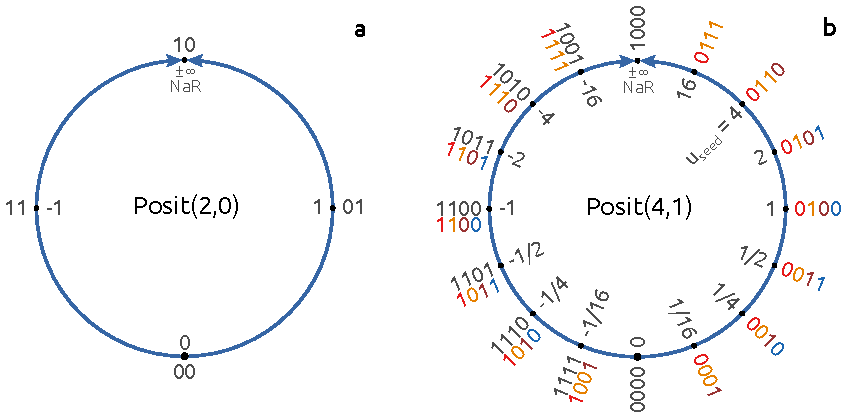
\includegraphics[width=1\textwidth]{figs/circles.pdf}
\caption{Two posit number formats obtained by projecting the real axis onto a circle. (a) 2bit Posit(2,0) and (b) 4bit Posit(4,1). The bit patterns are marked on the outside and the respective values on the inside of each circle. Bit patterns of negative numbers (black) have to be converted to their two's complement (colours) first (see text). At the top of every circle is complex infinity ($\pm \infty$) or NaR (Not-a-Real). After \citeA{Gustafson2017a}. }
\label{fig:circle}
\end{figure}

Posits also come with a no overflow/no underflow-rounding mode: Where floats overflow and return infinity when the exact result of an arithmetic operation is larger than the largest representable number ($maxpos$), posit arithmetic returns $maxpos$ instead, and similarly for underflow where the smallest representable positive number ($minpos$) is returned. This is motivated as rounding to infinity returns a result that is infinitely less correct than $maxpos$, although often desired to indicate that an overflow occurred in the simulation. Instead, it is proposed to perform overflow-like checks on the software level to simplify exception handling on hardware \cite{Gustafson2017a}. Many functions are simplified for posits, as only two exceptions cases have to be handled, zero and NaR. Conversely, Float64 has more than $10^{15}$ bitpatterns reserved for NaN, but these only make up $< 0.05\%$ of all available bit patterns. The percentage of redundant bitpatterns for NaN increases for floats with fewer exponent bits (Table \ref{tab:formats}), and only poses a noticable issue for Float16 and Float8.

The posit number framework also highly recommends \emph{quires}, an additional register on hardware to store intermediate results. Fused operations like \emph{multiply-add} can therefore be executed with a single rounding error without the rounding of intermediate results. The quire concept could also be applied to floating-point arithmetic, but is technically difficult to implement on hardware as the required registers would need to be much larger in size. For fair comparison we do not take quires into account. The posit number format is explained in more detail in \citeA{Gustafson2017a}. In order to use posits on a conventional CPU we developed for the Julia programming language \cite{Bezanson2017} the posit emulator \emph{SoftPosit.jl} \cite{Klower2019a}, which is a wrapper for the C-based library SoftPosit \cite{Leong2020}. The type-flexible programming paradigm,  facilitated by the Julia language, is outlined in \ref{sec:julia}.

\begin{figure}[htbp]
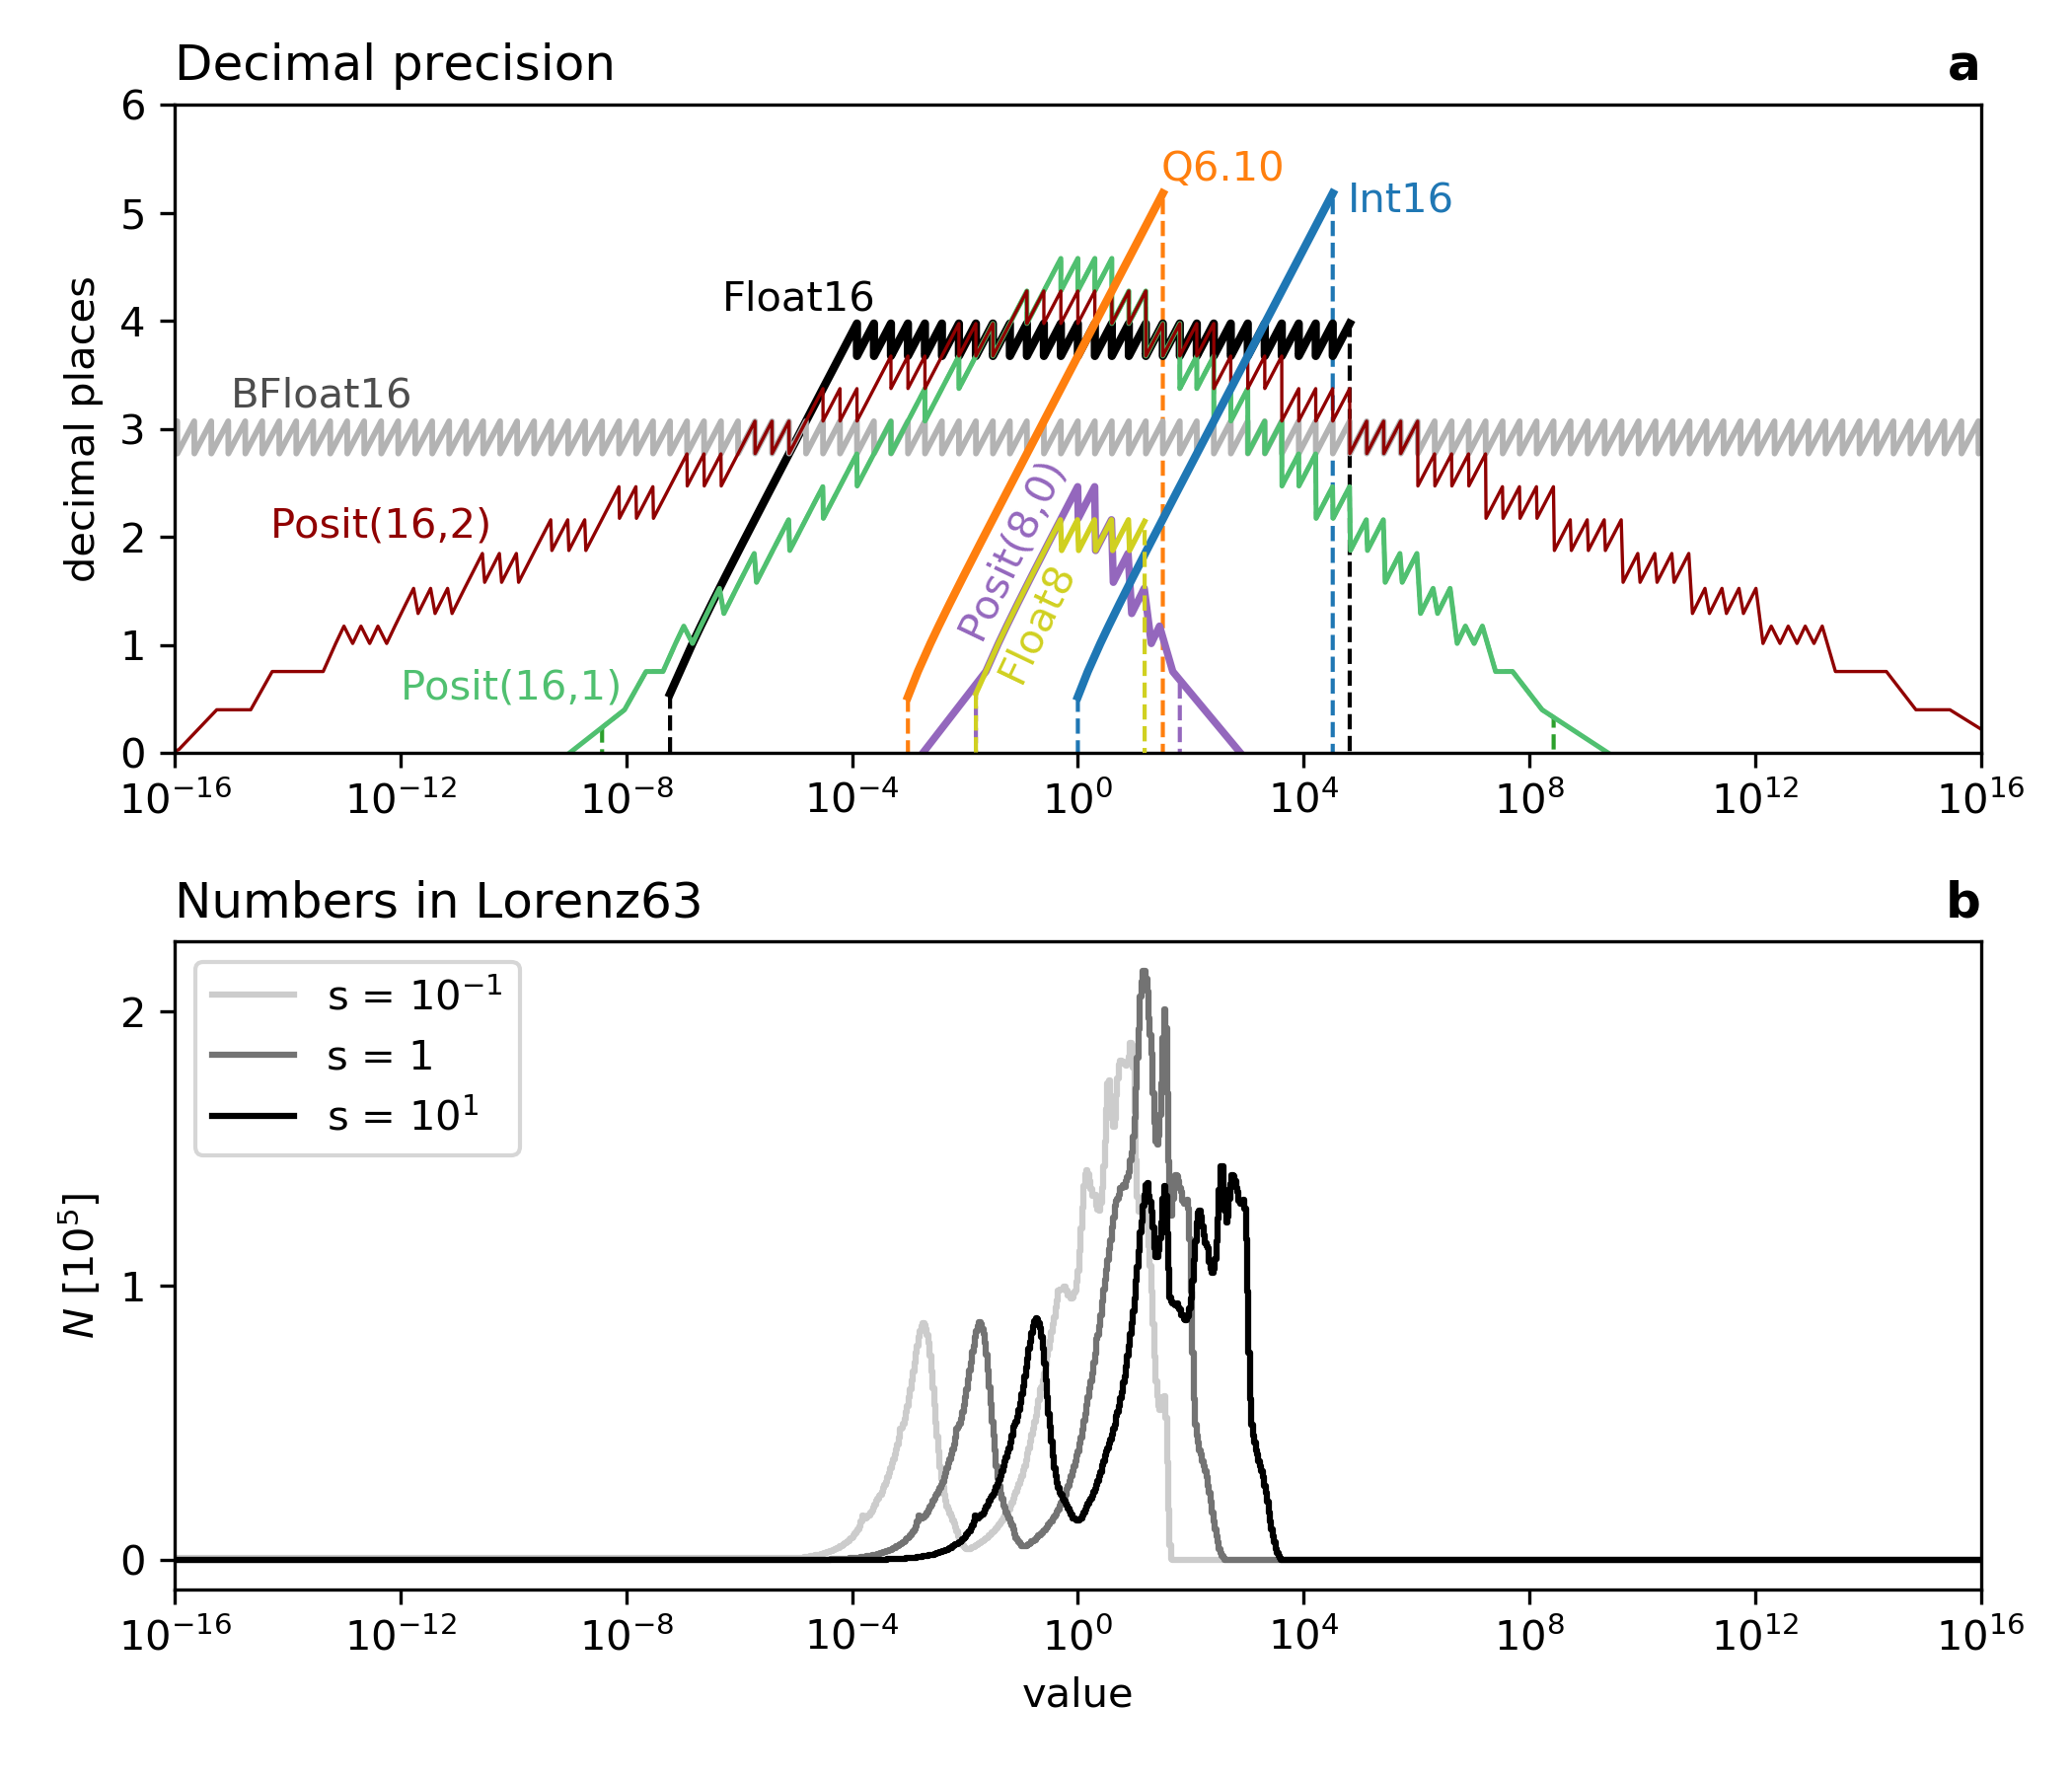
\includegraphics[width=1\textwidth]{../plots/decimal_precision.png}
\caption{(a) Decimal precision of various number formats. Dashed vertical lines indicate the range of representable numbers for each format. Float64, Float32 and Posit32 are beyond the axes limits. (b) Histogram of results of all arithmetic operations in the rescaled Lorenz system, considering absolute values.}
\label{fig:dec_acc}
\end{figure}

\subsection{Decimal precision}
\label{sec:decprec}

The decimal precision is defined as \cite{Gustafson2017,Gustafson2017a}
\begin{equation}
\op{decimal} \op{precision} = -\log_{10} \vert \log_{10}( \frac{x_\text{repr}}{x_\text{exact}} ) \vert
\end{equation}
where $x_\text{exact}$ is the exact result of an arithmetic operation and $x_\text{repr}$ is the representable number that $x_\text{exact}$ is rounded to, given a specified rounding mode. For the common round-to-nearest rounding mode, the decimal precision approaches infinity when the exact result approaches the representable number and has a minimum in between two representable numbers. This minimum defines the \emph{worst-case} decimal precision, i.e. the decimal precision when the rounding error is maximised. The worst-case decimal precision is the number of decimal places that are at least correct after rounding. 


Fig. \ref{fig:dec_acc}a compares the worst-case decimal precision for various 16 and 8bit floats and posits, as well as 16bit integers and the fixed-point format Q6.10 (6 integer bits, 10 fraction bits). Float16 has a nearly constant decimal precision of almost 4 decimal places, which decreases for the subnormal numbers towards the smallest representable number $minpos$. 16bit posits, on the other hand, show an increased decimal precision for numbers around 1 and a wider dynamic range, in exchange for less precision for numbers around $10^4$ as well as $10^{-4}$.  The machine error $\epsilon$, defined as half the distance between 1 and the next representable number, can be given in terms of decimal precision and is summarized in Table \ref{tab:formats} for the various formats. Due to the no overflow/no underflow-rounding mode, the decimal precision is slightly above zero outside the dynamic range. 

The decimal precision of 16bit integers is negative infinity for any number below 0.5 (round to 0) and maximised for the largest representable integer $2^{15} - 1 =  32767$. Similar conclusions hold for the fixed-point format Q6.10, as the decimal precision is shifted towards smaller numbers by a factor of $\tfrac{1}{2}$ for each additional fraction bit. Flexibility regarding the dynamic range can therefore be achieved with integer arithmetic if fixed point numbers are used \cite{Russell2017}. However, we did not achieve convincing results with integer arithmetic for the applications in this study, as rescaling of the equations is desired to place many arithmetic calculations near the largest representable number. However, any result beyond will lead to disastrous results, as integer overflow usually returns a negative value following a wrap-around behaviour. 


\section{Weather and climate models with 16bit arithmetics}


\subsection{The Lorenz 1963 system}
\label{sec:L63}

The Lorenz system (L63, \cite{Lorenz1963}) is a chaotic attractor and serves as a simplistic model for atmospheric convection. It is an extensively studied toy model for forecast uncertainty \cite{Lorenz1963,Kwasniok2014,Jeffress2017,Tantet2018} and is used here to investigate the accumulation of rounding errors in the numerical integration of a chaotic system. The Lorenz system consists of the variables $x$,$y$ and $z$ that are described by the following non-linear differential equations
\begin{subequations}
\begin{align}
\frac{dx}{dt} &= \sigma(y-x) \\
\frac{dy}{dt} &= x(\rho - z) - y \\
\frac{dz}{dt} &= xy - \beta z
\end{align}
\label{eq:L63}%
\end{subequations}
with the typical parameter choices $\sigma = 10, \rho = 28$ and $\beta = \tfrac{8}{3}$, that permit chaotic behaviour. 

\begin{figure}
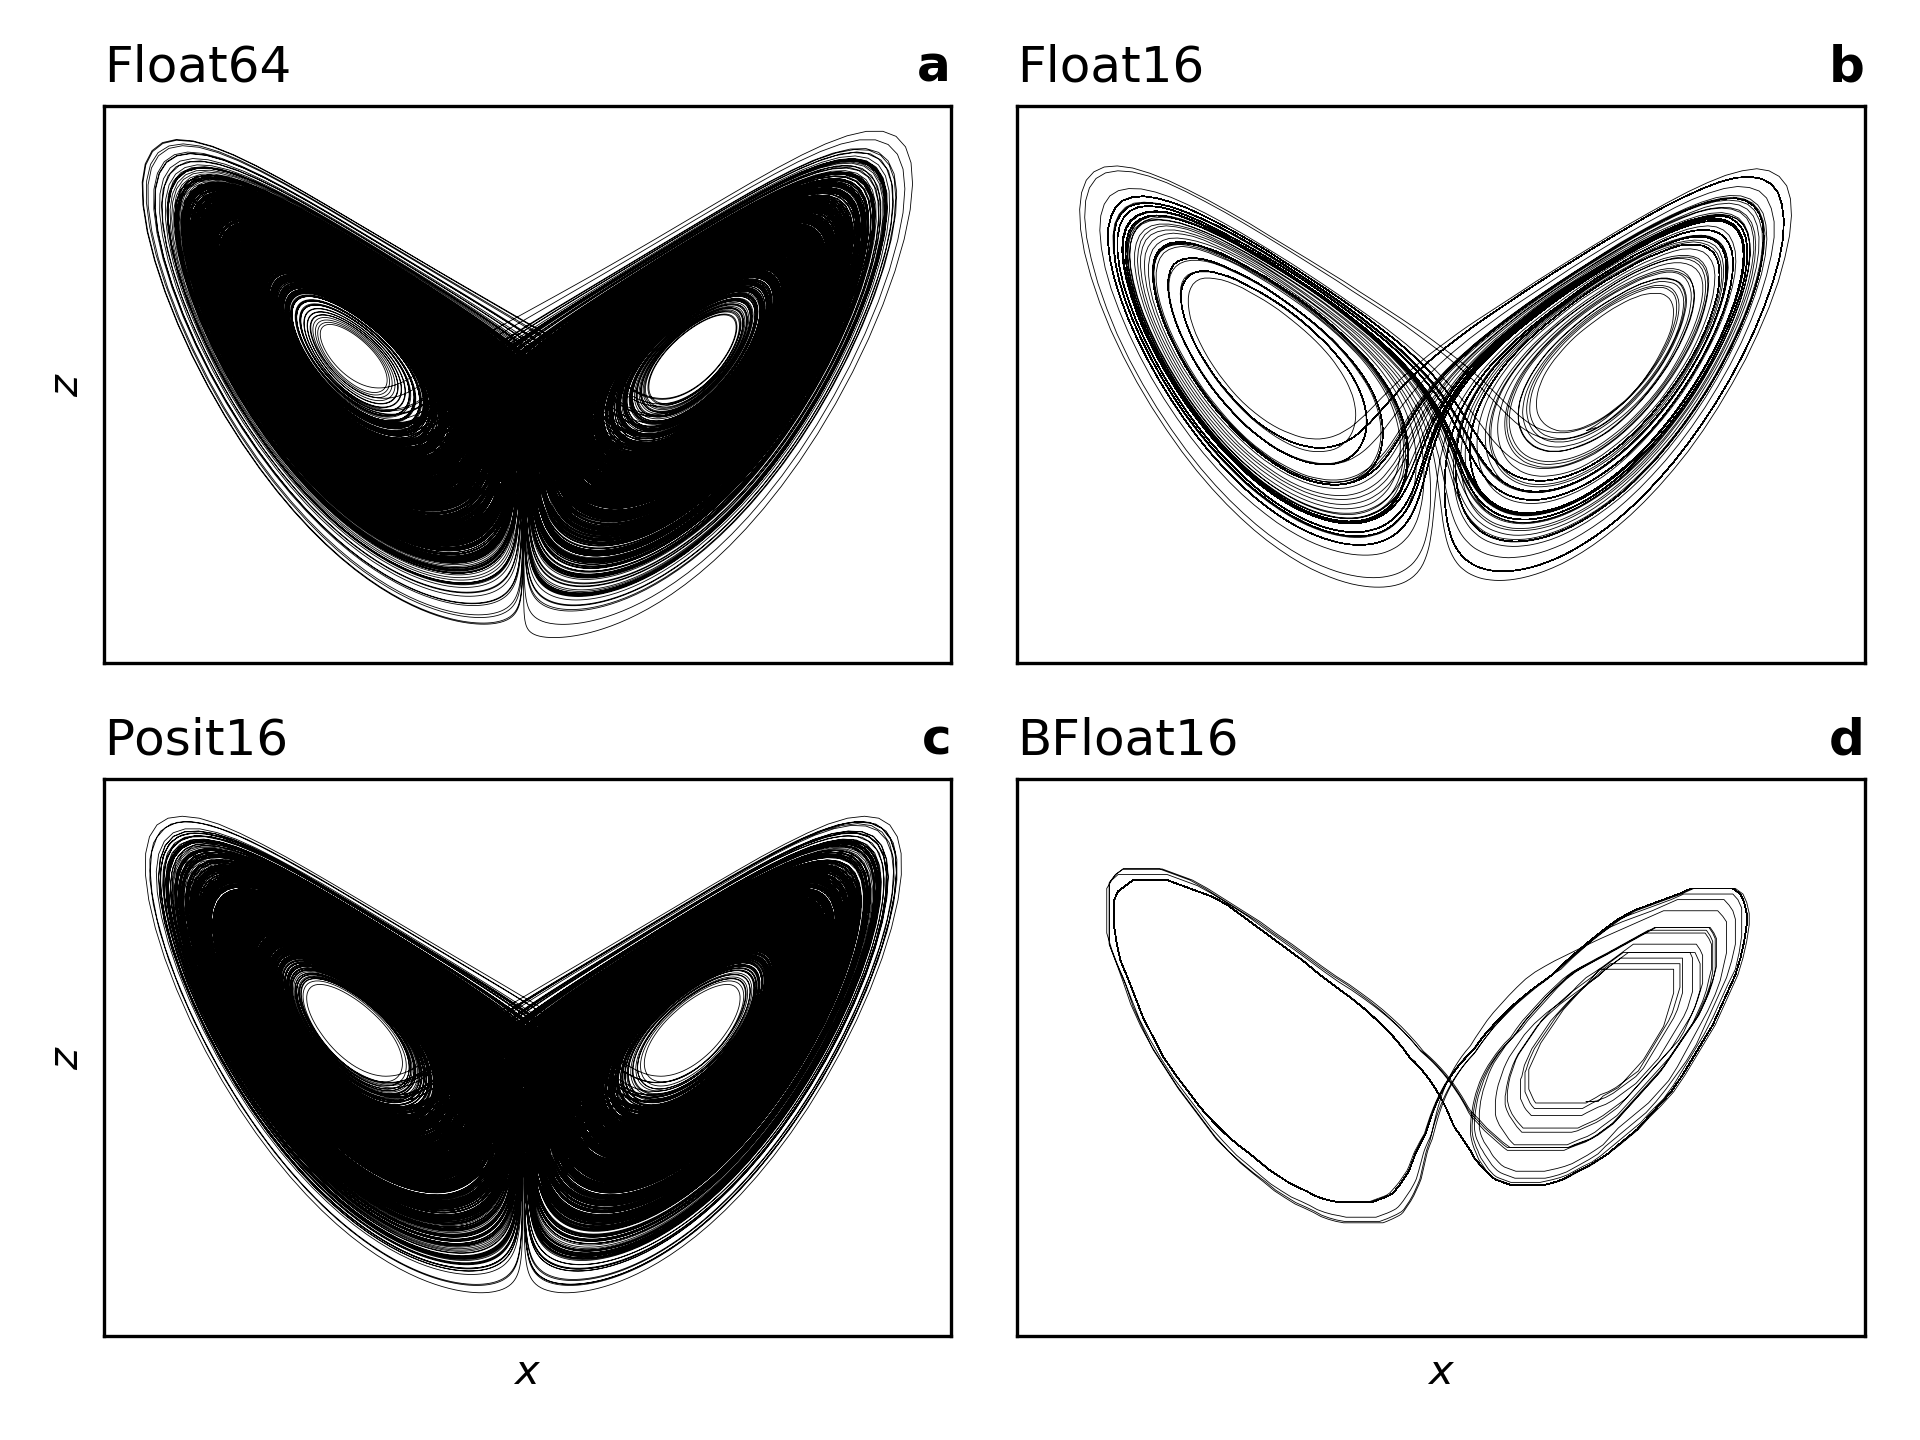
\includegraphics[width=1\textwidth]{../plots/lorenz_attractor.png}
\caption{The Lorenz attractor computed with different number formats. The scaling of the Lorenz equations (Eq. \ref{eq:L63s}) is (a,b,d) $s=1$, (c) $s=0.1$. All trajectories are integrated from the same initial conditions for 100,000 time steps with spacing $\Delta t = 0.008$.}
\label{fig:L63}
\end{figure}

Regardless of the initial conditions, the Lorenz system will evolve towards a set of $(x,y,z)$ points called attractor (the x,z-section of the attractor is shown in Fig. \ref{fig:L63}a). This attractor is \emph{strange}, i.e. its geometric structure cannot be described in two dimensions, but is of fractal nature. While points on the model trajectory will get infinitesimally close to each other, the trajectory of the analytical Lorenz system will never repeat itself. However, if the model is discretised and if the variables are represented with finite precision, only a finite amount of distinct states can be represented and the model trajectory will eventually repeat itself if integrated for long enough. 

Integrating the Lorenz system with Float16 yields an attractor that is repeating itself fairly early and the space that is filled by the line of the trajectory is significantly smaller when compared to the space of a trajectory with double precision (compare Fig. \ref{fig:L63}a and b). However, when using Posit(16,1) and a rescaling factor of $s=0.1$ (see section \ref{sec:L63_rescale}) the representation of the attractor is improved significantly (Fig. \ref{fig:L63}c). The results for posits look similar to the results with Float16 if no rescaling was used (not shown here). Only a time step $\Delta t > 0.008$ yields tendencies that are large enough to overcome the rounding errors of BFloat16 that otherwise inhibit a temporal evolution of the system. Although a time step of 0.008s allows the Lorenz system to be integrated with BFloat16, only a poor representation of the fractal attractor is achieved (Fig. \ref{fig:L63}d). The solution of the Lorenz system with 16bit integers presents a similarly simple Lorenz attractor \cite{Klower2019}.

\subsection{Shallow water model}
\label{sec:swm}

This section will evaluate the different number formats Float16, BFloat16, Posit(16,1) and Posit(16,2) when solving the shallow water equations. The shallow water equations result from a vertical integration of the Navier-Stokes equations under the assumption that horizontal length scales are much greater than vertical scales. This assumption holds for many features of the general circulation of atmosphere and ocean \cite{Gill1982,Vallis2006}. The shallow water equations for the prognostic variables velocity $\mathbf{u} = (u,v)$ and sea surface elevation $\eta$ are
\begin{subequations}
\begin{align}
\frac{\partial \mathbf{u}}{\partial t} &+ (\mathbf{u} \cdot \nabla) \mathbf{u} + f\hat{\mathbf{z}} \times \mathbf{u} = -g\nabla \eta + \mathbf{D} + \mathbf{F} \\
\frac{\partial \eta}{\partial t} &+ \nabla \cdot (\mathbf{u}h) = 0.
\end{align}
\label{eq:swe}%
\end{subequations}
For the atmosphere, $\eta$ is interpreted as pressure \cite{Gill1982}. The shallow water system is forced with a zonal wind stress $\mathbf{F}$. The dissipation term $\mathbf{D}$ removes energy on large scales (bottom friction) and on small scales (diffusion). The non-linear term $(\mathbf{u} \cdot \nabla) \mathbf{u}$ represents advection of momentum. The term $f\hat{\mathbf{z}} \times \mathbf{u}$ is the Coriolis force and $-g\nabla \eta$ is the pressure gradient force, with $g$ being the gravitational acceleration. Eq. \ref{eq:swe}b is the shallow water-variant of the continuity equation, ensuring conservation of mass. 

The shallow water equations are solved in the $(x,y)$-plane over the zonally periodic rectangular domain $L_x \times L_y$, of size $2000\op{km} \times 1000\op{km}$, with a meridional mountain ridge in the middle of the domain. We associate $x$ with the zonal and $y$ with the meridional direction. The domain is centred at 45N and the beta-plane approximation \cite{Vallis2006} is used to linearize the Coriolis parameter which varies linearly from $7.27 \times 10^{-5}\op{s}^{-1}$ at the southern boundary to $9.25 \times 10^{-5}\op{s}^{-1}$ at the northern boundary. The boundary conditions are periodic in zonal direction and no-slip at the northern and southern boundary. The layer thickness is $h = \eta + H(x)$, with
\begin{equation}
H(x) = H_0 - H_1\exp\left(-H_\sigma^{-2}(x-\tfrac{L_x}{2})^2\right)
\end{equation}
being the undisturbed depth, representing a mountain ridge at $x=\tfrac{L_x}{2}$ spanning from the southern to the northern boundary. The standard depth is $H_0 = 500\op{m}$. The ridge has a height of $H_1 = 50\op{m}$. The characteristic width of the ridge is $H_\sigma = 300\op{km}$. The time step $\Delta t = 282\op{s}$ is chosen to resolve surface gravity waves, traveling at maximum phase speed $\sqrt{gH_0}$ with CFL number being close to 1 and gravitational acceleration $g=10\op{ms}^{-1}$. The wind stress forcing $\mathbf{F} = (F_x,0)$ is constant in time, acts only on the zonal momentum budget
\begin{equation}
Fx = \frac{F_0}{\rho h} \cos\left(\pi\left(y{L_y}^{-1} - 1\right)\right)^2
\end{equation}
and vanishes at the boundaries. The water density is $\rho = 1000\op{kg}\op{m}^{-3}$ and $F_0 = 0.12\op{Pa}$. The dissipation term $\mathbf{D}$ is the sum 
\begin{equation}
\mathbf{D} = -\frac{c_D}{h}\| \mathbf{u} \| \mathbf{u} - \nu \nabla^4 \mathbf{u}
\label{eq:diss}
\end{equation}
of a quadratic bottom drag with dimensionless coefficient $c_D = 10^{-5}$ \cite{Arbic2008} and a biharmonic diffusion with viscosity coefficient $\nu \approx 1.33\times10^{11} \op{m}^4\op{s}^{-1}$ \cite{Griffies2000}. 

The shallow water equations are discretised using 2nd order centred finite differences on an Arakawa C-grid \cite{Arakawa1977} with a grid spacing of $\Delta = 20\operatorname{km}$ (100x50 grid points) and the Runge-Kutta fourth order method \cite{Butcher2016} is used for time integration of the pressure, coriolis and advective terms, whereas a semi-implicit method is used for the dissipative terms $\mathbf{D}$. The advection terms are discretised using an energy and enstrophy conserving scheme \cite{Arakawa1990}. 

To test the use of the different number formats for the representation of passive tracers in atmosphere and ocean, we extend the shallow water equations with an advection equation. Tracers could, for example, be temperature and salinity in the ocean or aerosols in the atmosphere, which are regarded here, for simplicity, as passive (i.e. they do not influence the flow). The change of the distribution of a passive tracer $q$ that is advected by the underlying flow field is described by
\begin{equation}
\frac{\partial q}{\partial t} + \mathbf{u} \cdot \nabla q = 0.
\label{eq:adv}
\end{equation}
We discretise Eq. \ref{eq:adv} with a semi-Lagrangian advection scheme \cite{Smolarkiewicz1992}, which calculates the tracer concentration for a given grid cell from the concentration at the previous time step at a departure point, which in turn is determined from the flow field. As the departure point is in general in between grid nodes an interpolation is required to find the concentration at the departure point.

We change the algorithms in the shallow water model slightly by employing techniques of rescaling, reordering and precomputing to make the computations more suitable for the limitations of 16bit arithmetics. Some of these techniques are discussed in section \ref{sec:rescale}.

\subsection{16bit shallow water simulations}

\begin{figure}
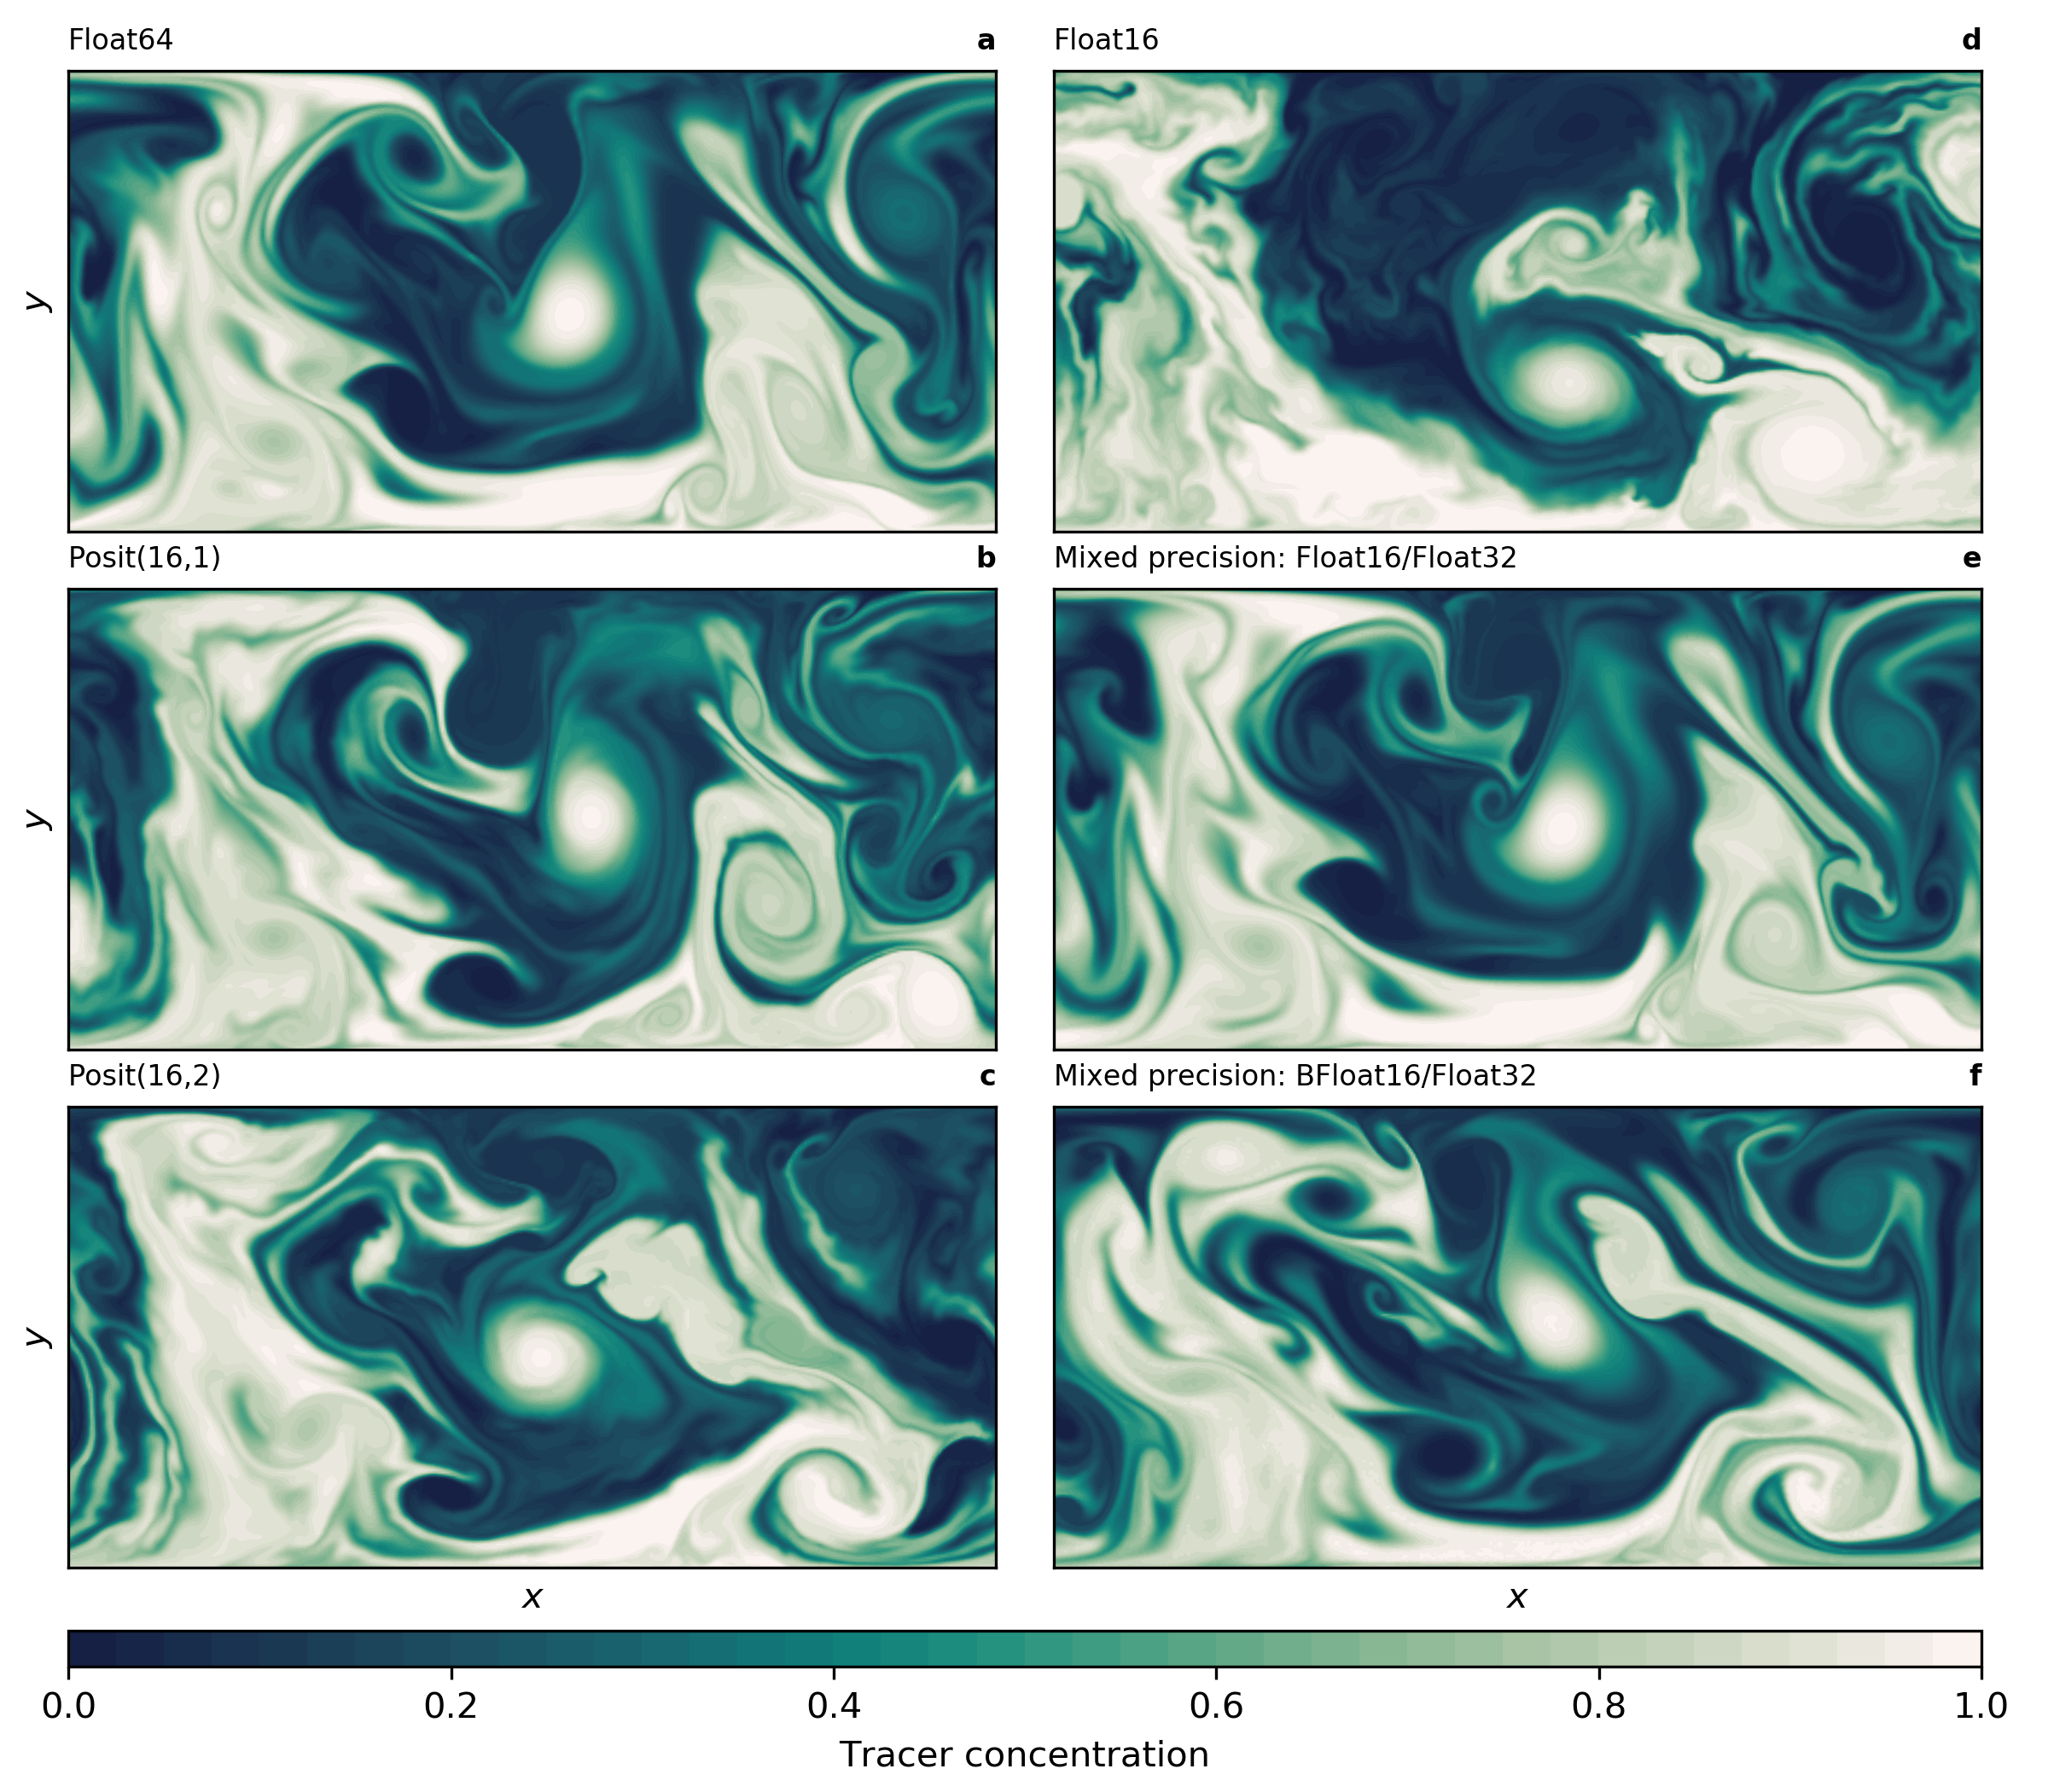
\includegraphics[width=1\textwidth]{../plots/snapshot.png}
\caption{Snapshot of tracer concentration simulated by the shallow water model using different 16bit number formats. Mixed precision using Float32 for the prognostic variables only is used for (e) and (f). The tracer was injected uniformly in the lower half of the domain 50 days before. This simulation was run at an increased resolution of $\Delta = 5$km (400x200 grid points).}
\label{fig:snapshot}
\end{figure}

The solution to the shallow water equations includes vigorous turbulence that dominates a meandering zonal current. Using either float or posit arithmetic in 16 bit the simulated fluid dynamics are very similar to a Float64 reference: As shown in a snapshot of tracer concentration (Fig. \ref{fig:snapshot}) turbulent stirring and mixing can be well simulated with posits. However, the Float16 simulation (Fig. \ref{fig:snapshot}d) deviates much faster than the posit simulations (Fig. \ref{fig:snapshot}b and c) from the Float64 reference (Fig. \ref{fig:snapshot}a), presumably due to the small scale instabilities visible in the snapshot as wavy filaments and fronts. These instabilities are clearly triggered by Float16 arithmetics, but to a lower degree also visible for posits. This provides a first evidence that the accumulated rounding errors with posits are smaller than with floats. BFloat16 arithmetic is not able to simulate the shallow water dynamics, presumably as tendencies are too small to be added to the prognostic variables, an issue that also occurs in the Lorenz system (Fig. \ref{fig:L63}d) and even in the harmonic sum (Fig. \ref{fig:harmsum2}).

\begin{figure}
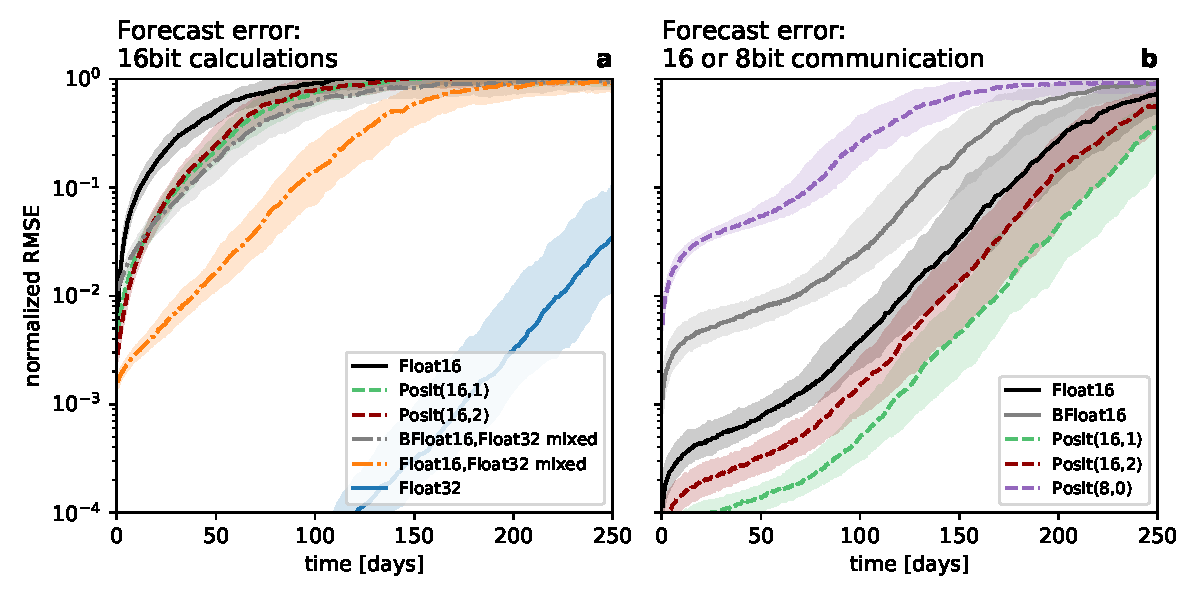
\includegraphics[width=1\textwidth]{../plots/rmse_eta.pdf}
\caption{Forecast error measured as the root mean square error (RMSE) of sea surface height $\eta$ taking Float64 as reference. (a) Forecast error for various 16bit number formats and mixed 16bit/32bit simulations for which the prognostic variables are kept at Float32. (b) Forecast error for reduced precision communication in 8 or 16bit with various number formats used for encoding, with Float64 used for all calculations.  The communication of boundary values occurs at every time step for the prognostic variables. The RMSE is normalised by a mean forecast error at very long lead times. Solid lines represent the median of 200 forecasts per number format. The shaded areas of each model configuration denote the interquartile range of the ensemble.}
\label{fig:rmse}
\end{figure}

To quantify differences between the different 16bit arithmetics we perform ensemble forecasts. Some initial conditions describe a more predictable state of the shallow water system than others. To quantify the error growth of rounding errors with different arithmetics in a statistically robust way, we create an ensemble of forecasts with each member starting from one of 200 randomly picked start dates from a 50 year long control simulation. The forecast error in the shallow water model is computed as root mean square error (RMSE) of sea surface height with respect to Float64. Other variables yield similar results. Each forecast is performed several times from identical initial conditions but with the various number formats. To compare the magnitude of rounding error that are caused by a reduction in precision to a realistic level of error that is caused by model discretisation, we also perform forecasts with Float64 at half the spatial resolution $\Delta = 40~\op{km}$. We normalise the RMSE by the climatological mean forecast error at very long lead times, which is the same for all model configurations. A normalised RMSE of 1 therefore means that all information of the initial conditions is removed by chaos.

The forecast error of Float16 is as large as the discretisation error and clearly outperformed by 16bit posit arithmetic (Fig. \ref{fig:rmse}a). Both Posit(16,1) and Posit(16,2) yield a forecast error that is several times smaller than Float16. The forecast error of 32bit arithmetic is several orders of magnitude smaller and is only after 200 days as large as the error for 16bit arithmetic at very short lead times. Also at 32bit, posits clearly outperform floats.

\begin{figure}
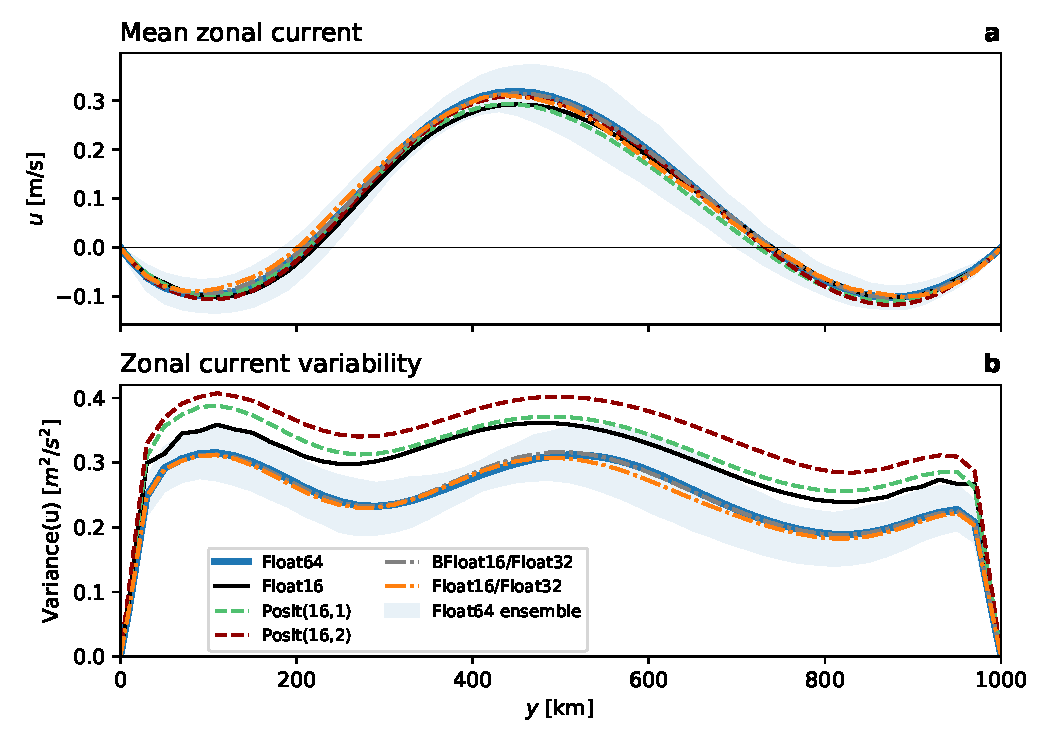
\includegraphics[width=1\textwidth]{../plots/meanvar_u.pdf}
\caption{Climatology and variability of the zonal current. (a) Zonally-averaged zonal current $u$ as a function of the meridional coordinate $y$. (b) Zonal variance of the zonal current as a function of $y$. The shaded area denotes the interquartile temporal variability around the (a) mean and (b) variance of reference simulation with Float64.}
\label{fig:mean}
\end{figure}

To investigate the effect of rounding errors on the climatological mean state of the shallow water system, we zonally average the zonal velocity $u$. The mean state is an eastward flow of about 0.3~m/s, about 3 to 4 times weaker than individual velocities throughout the domain (Fig. \ref{fig:mean}a), which is typical for turbulent flows. A weak westward mean flow is found at the northern and southern boundary. No 16bit format was found to have a significant impact on the mean state. The variability of the flow around its mean state is high throughout the domain (Fig. \ref{fig:mean}b). The variability is significantly increased by 10 -- 30\% with 16bit arithmetic, especially with Posit(16,2). The increased rounding errors with 16bit arithmetic likely trigger instabilities in the flow, which grow and subsequently explain the increased variability.

\begin{figure}
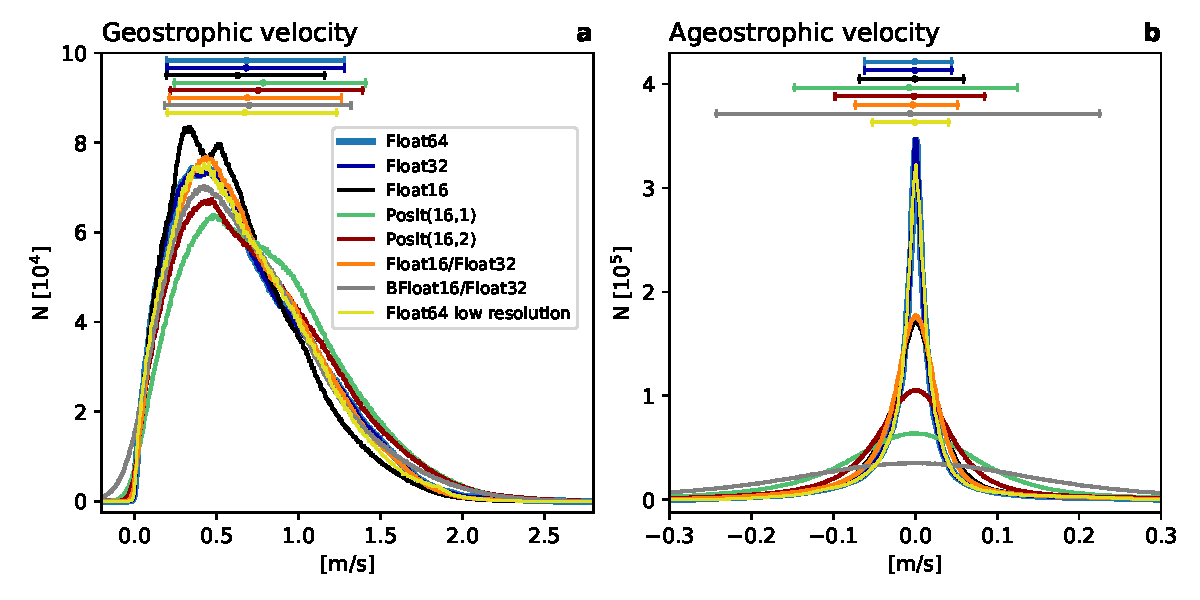
\includegraphics[width=1\textwidth]{../plots/ageostrophic.pdf}
\caption{Geostrophic balance as simulated with different number formats. (a) Histograms of flow-parallel components of geostrophic velocity. (b) as (a) but for the ageostrophic velocities. Horizontal bars denote the mean, 10th and 90th-percentile in respective colours.}
\label{fig:geo}
\end{figure}

The turbulence in shallow water simulations is largely geostrophic, such that the pressure gradient force opposes the Coriolis force. The resulting geostrophic velocities $\mathbf{u}_g$ can be derived from the sea surface height $\eta$
\begin{subequations}
\begin{align}
\mathbf{u}_g &= \frac{g}{f}\hat{\mathbf{z}} \times \nabla \eta \\
\mathbf{u} &= \mathbf{u}_{g} + \mathbf{u}_{ag}
\end{align}
\label{eq:geo}%
\end{subequations}
and deviations from the actual flow $\mathbf{u}$ are the ageostrophic velocity components $\mathbf{u}_{ag}$. We project both components on the actual velocities to obtain the flow-parallel components $\tilde{u}_{g}$ and $\tilde{u}_{ag}$ via
\begin{equation}
\tilde{u}_g = \frac{\mathbf{u}_g \cdot \mathbf{u}}{\| \mathbf{u} \|}, \quad \tilde{u}_{ag} = \frac{\mathbf{u}_{ag} \cdot \mathbf{u}}{\| \mathbf{u} \|}.
\label{eq:parallel}%
\end{equation}
The geostrophic velocities in the shallow water simulations can reach up to 2 m/s, are virtually never negative (i.e. against the flow) and have a mean of about 0.7 m/s (Fig. \ref{fig:geo}a). This behaviour is well simulated with 16bit number formats, although posits increase the strength of geostrophic velocities slightly. Ageostrophic velocity components are found to be isotropic, and are oriented equally frequent with and against the prevailing flow, but rarely exceed $\pm$0.1m/s and are therefore comparably small as expected in geostrophically balanced turbulence. Ageostrophic velocities can be seen as a measure of the physical instabilities in the flow field and their variance is indeed increased when simulated with 16bit number formats. Float16 shows clearly fewer ageostrophic velocities around 0, pointing towards an increased number of simulated instabilities. Posits have an even further increased number of ageostrophic velocities, and especially Posit(16,1) increases the variance of those by more than factor of two. It is unclear where in the model integration rounding errors of 16bit arithmetic trigger instabilities that lead to the observed increase in ageostrophy. We conclude that although the geostrophic balance in the simulations is maintained, rounding errors lead, likely due to an increase in ageostrophy, to a higher variability in the flow field. As the tracer field simulated by Float16 includes recognizably more small scale variablity compared to posits, it follows that some of this variability might actually be geostrophically balanced. 

\begin{figure}
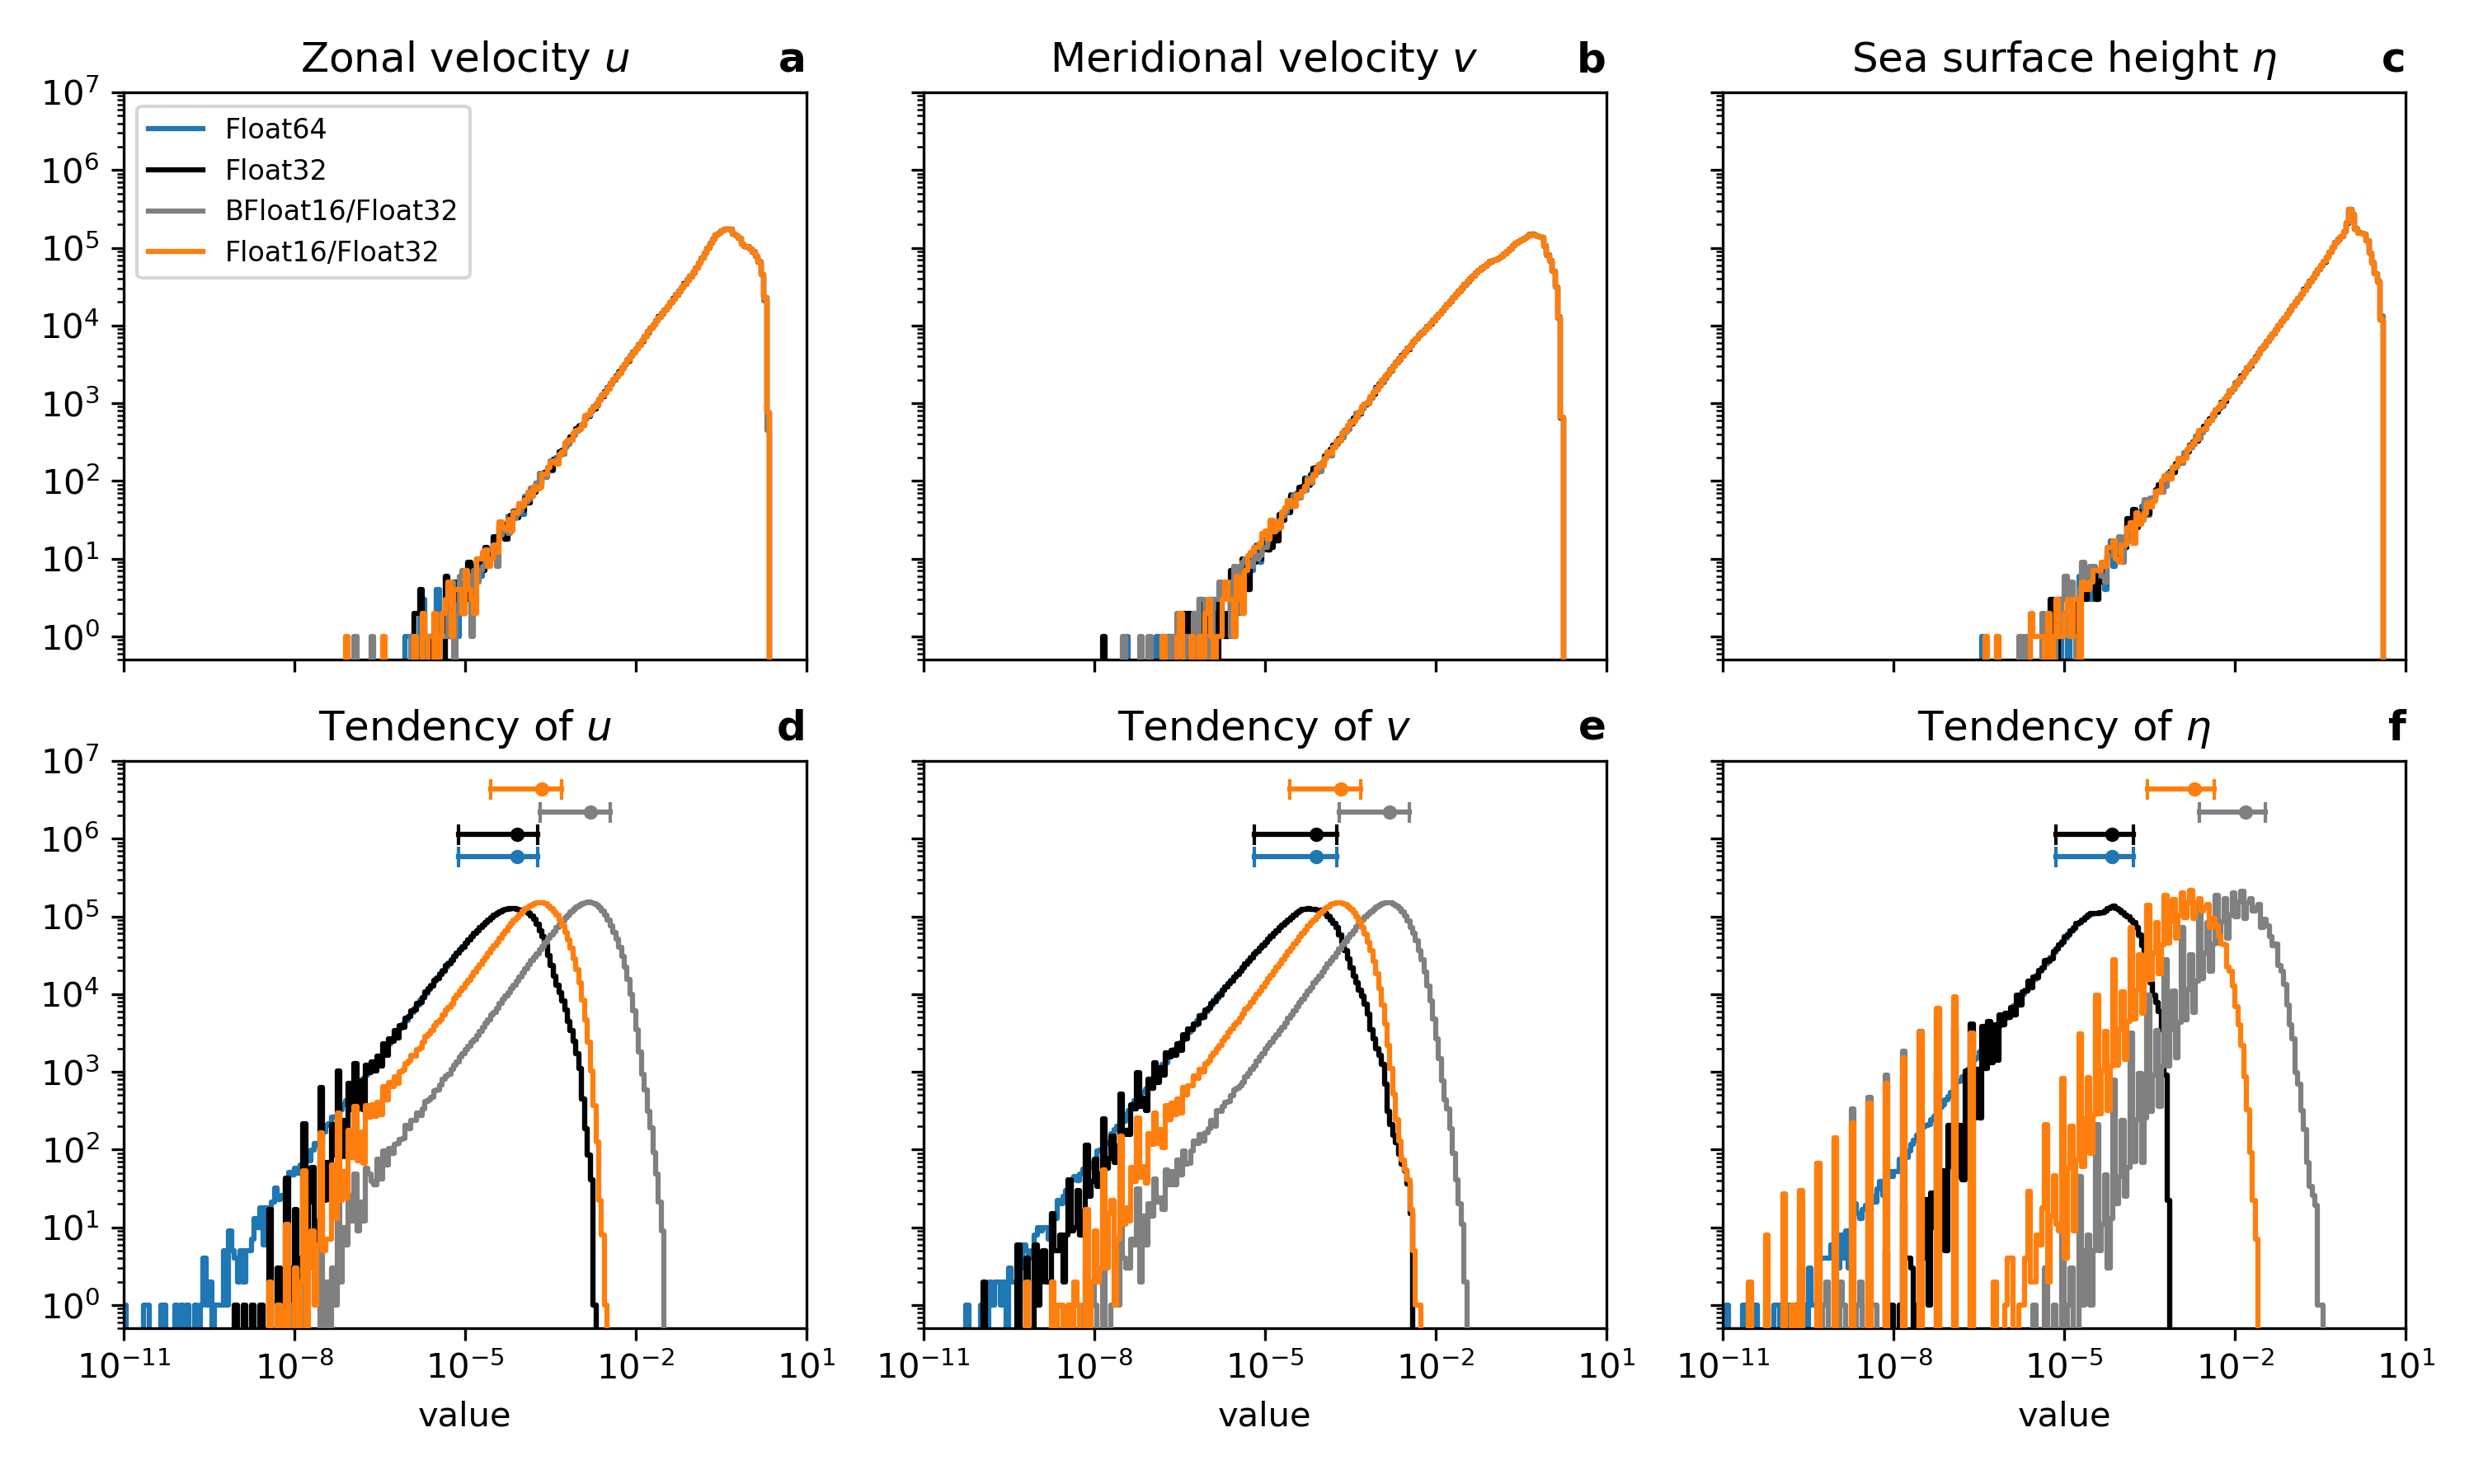
\includegraphics[width=1\textwidth]{../plots/tendency_hist.png}
\caption{Histograms of the numeric values of the prognostic variables (a) zonal velocity $u$, (b) sea surface height $\eta$, and the respective tendencies of (d) $u$ and (e) $\eta$, simulated with different 16, 32 and 64bit number formats. Mean, 10th and 90th percentile are shown above the histograms in respective colors. Snapshots of the tendencies of $\eta$ simulated with (c) Float64 and (f) Posit(16,1), other 16bit formats are similar. Areas of sea surface height anomalies exceeding $\pm1.4$~m are shown in purple (negativ) and yellow (positive). Note the break on the x-axis in (a,b,d) and (e).}
\label{fig:tend}
\end{figure}

As 16bit arithmetics have no significant impact on the climatological mean state, histograms of prognostic variables are also not changed (Fig. \ref{fig:tend}a and b). However, the tendencies are increased by orders of magnitude with 16bit arithmetics (Fig. \ref{fig:tend}d and e), as rounding errors cause gravity waves to radiate away from eddies (Fig. \ref{fig:tend}f). Gravity waves are identified from the tendency of sea surface height. Comparing their propagation to the location of anomalous sea surface height, which is used as a proxy for eddies, we assume that rounding errors in regions of high eddy activity lead to instabilities that propagate away in the form of gravity waves. These gravity waves are not present in Float64 simulations (Fig. \ref{fig:tend}c) and tend to have only a small impact on quasi-gestrophic dynamics, as they act on different time and length scales. It is unclear whether these gravity waves cause the observed ageostrophic velocities. 

The tendencies are about 4 orders of magnitude smaller than the prognostic variables. This poses a problem for number formats with a machine error, measured as decimal precision, significantly lower than 4 decimal places (Table \ref{tab:formats}). Float16 has a machine error of 3.7, which is presumably close to the lower limit beyond which the addition of tendencies will be round back, an effect already observed for the harmonic sum. The BFloat16 number format has a machine error of 2.8, which explains why no change from initial conditions in the shallow water system can be simulated with BFloat16.

\section{Mixed precision arithmetic}
\label{sec:mixed}

In the previous section the entire shallow water simulation was performed with the specified number format. As the addition of tendencies to the prognostic variables was identified as a key calculation that is error-prone, we investigate now the benefits of mixed precision arithmetic, where Float32 is used for the prognostic variables but the tendencies are computed with either Float16 or BFloat16, two number formats that have the lowest decimal precision for numbers around 1. The prognostic variables are now reduced to Float16 or BFloat16 before calculations of the right-hand side and every term of the tendencies is converted back before addition to the prognostic variables. Using subscripts 16 and 32 to denote variables held at 16 and 32bit precision, respectively, and let Float32() be the conversion function then the continuity Eq. \ref{eq:swe}b becomes
\begin{equation}
\frac{\partial \eta_{32}}{\partial t} = -\op{Float32}( \partial_x(u_{16}h_{16}) + \partial_y(v_{16}h_{16} ))
\label{eq:conversion}
\end{equation}
and similar for $u$ and $v$ in Eq. \ref{eq:swe}a.

Snapshots of tracer concentration reveal well simulated geostrophic turbulence (Fig. \ref{fig:snapshot}e and f) with Float16/Float32 or BFloat16/Float32 and instabilites at fronts or in filaments are visibly reduced compared to pure 16bit arithmetic. The forecast error is strongly reduced once the prognostic variables are kept as Float32 (Fig. \ref{fig:rmse}a), supporting the hypothesis that the addition of tendencies to the prognostic variables is a key computation with low rounding error-tolerance. Despite BFloat16 not being suitable for shallow water simulations when applied to all computations, mixing BFloat16 with Float32 arithmetic yields a similar error growth to posits, which is well below the discretization error. Mean state or variability are virtually identical for both mixed precision cases (Fig. \ref{fig:mean}) compared to the Float64 reference. The geostrophic balance is largely unaffected, but ageostrophic velocities increase in variance, especially for BFloat16 (Fig. \ref{fig:geo}). Gravity waves are similarly present for mixed precision although weaker for tendencies computed with Float16 (Fig. \ref{fig:tend}d) and, as discussed, they tend to not interact with the geostrophic time and length scales. Although the results show that Float16 is generally a preferrable number format over BFloat16 for the applications presented here, we acknowledge that the conversion between Float32 and Float16 will come with some computational cost. In contrast, the conversion between BFloat16 and Float32 is computationally very cheap as both formats have the same number of exponent bits. Removing signifcant bits, potentially applying rounding, and padding trailing zeros, are the only operations for this conversion. Following the results here, mixing 16 and 32bit precision is found to be a possible solution to circumvent roundings errors with 16bit floating-point arithmetics. Performance benefits are still possible as most calculations are performed with 16bit, with key computations in 32bit to reduce the overall error. Depending on the application, the conversions between number formats are assumed to be of negligible cost. This is an attractive solution as hardware-accelerated 16bit floating-point arithmetic is already available on graphic or tensor processing units and implementations therefore do not rely on the development of future computing hardware, as it is the case for posits.

\begin{figure}
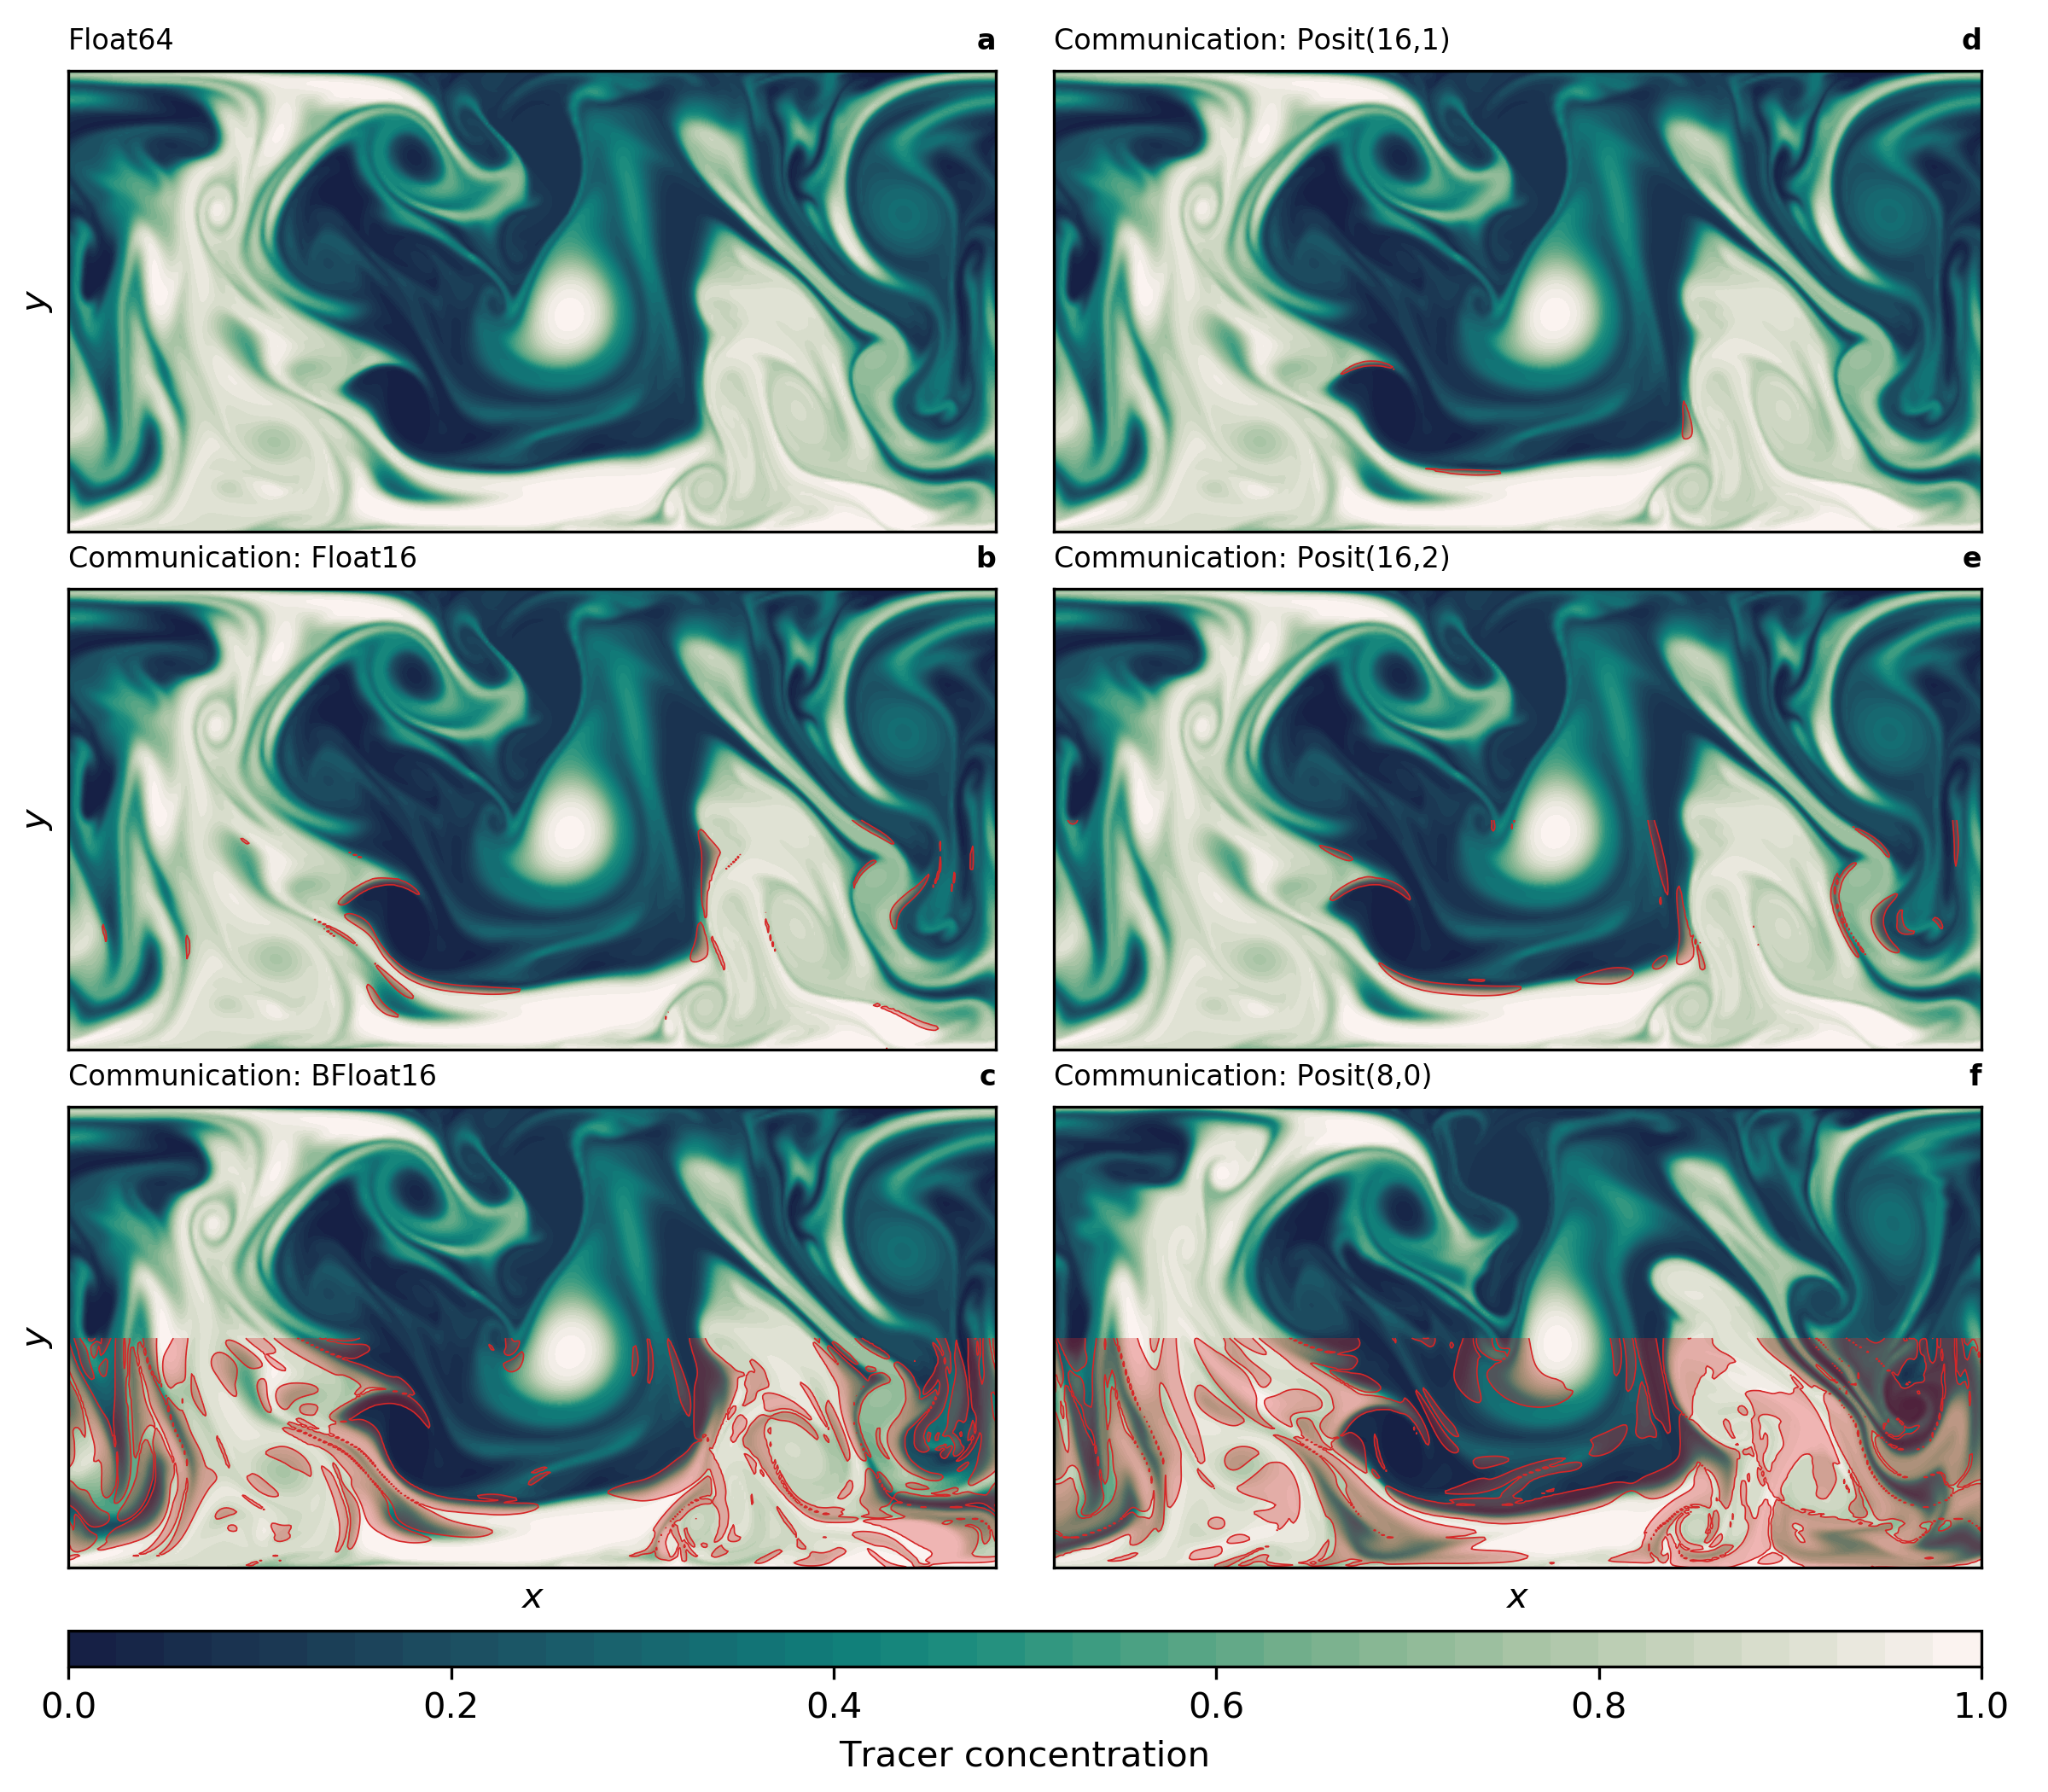
\includegraphics[width=1\textwidth]{../plots/snapshot_comm.png}
\caption{Snapshot of tracer concentration simulated by the shallow water model using reduced precision communication. The communication of boundary values occurs at every time step for the prognostic variables. Float64 was used for all calculations. Areas where the absolute error exceeds 0.05 are shaded in red only in the lower half of the domain. The tracer was injected uniformly in the lower half of the domain 50 days before. This simulation was run at a resolution of $\Delta = 5$km (400x200 grid points).}
\label{fig:snapshot_comm}
\end{figure}

\section{Algorithmic changes: Rescaling, reordering and precomputations}
\label{sec:rescale}

\subsection{Rescaling the Lorenz 1963 system }
\label{sec:L63_rescale}

It is possible to influence the range of numbers occuring in arithmetic operations in an algorithm using a \emph{rescaling} of the equations via a simple multiplication of the variables with a constant rescaling factor $s$. For the Lorenz 1963 system (Eq. \ref{eq:L63}, the rescaled variables are denoted as $\tilde{x} = sx$, and similarly for $\tilde{y},\tilde{z}$. Fig. \ref{fig:dec_acc}b shows histograms for all numbers that are used to solve the Lorenz system (including intermediate calculations). A comparison to the decimal precision in Fig. \ref{fig:dec_acc}a reveals the benefit of rescaling, especially for posit arithmetic: To profit from the increased decimal precision around 1, a scaling with $1/10$ is proposed to shift most calculations towards the centre of the dynamic range of representable numbers. Due to the constant decimal precision for floats, rescaling is less relevant for float arithmetic as long as no overflow nor underflow occurs. For integers, on the other hand, the Lorenz equations should be upscaled by a factor of approximately $100$, to shift the range of numbers to a higher decimal precision.

We solve the equations using a fourth order Runge-Kutta method \cite{Butcher2016}. Each substep in the time integration can be written as 
\begin{subequations}
\begin{align}
\tilde{x}^{n+1} &= \tilde{x}^n + RK_x\left(\tilde{y}^n-\tilde{x}^n\right) \\
\tilde{y}^{n+1} &= \tilde{y}^n + RK_y\left(\tilde{x}^n(\rho - \frac{\tilde{z}^n}{s}) - \tilde{y}^n \right) \\
\tilde{z}^{n+1} &= \tilde{z}^n + RK_z\left(\tilde{x}^n\frac{\tilde{y}^n}{s} - \beta \tilde{z}^n\right)
\end{align}
\label{eq:L63s}%
\end{subequations}
where $RK_x,RK_y,RK_z$ contain the Runge-Kutta coefficient and the time step $\Delta t$.  $RK_x$ also contains the parameter $\sigma$. The superscripts $n$ and $n+1$ denote the current and next time substep.

The rescaling of the Lorenz system has its limitations: The non-linear terms in Eq. \ref{eq:L63s} involve a division by the scaling constant $s$, which leads to the result of the arithmetic operations $\tfrac{\tilde{z}}{s}, \rho - \tfrac{\tilde{z}}{s},$ and $\tfrac{\tilde{y}}{s}$ being invariant under scaling. This is observed in the histograms of arithmetic results (Fig. \ref{fig:dec_acc}b), as high counts of values between 1 and 50 exist for different choices of $s$. A changing shape of the histogram with $s$ is a consequence. Following these results an underlying challenge of reduced precision modelling becomes apparent: One has either to find a number format that fits the range of computed numbers, or rescale the equations to optimise their range for a given number format.

\subsection{Rescaling the shallow water equations}
\label{sec:swm_rescale}

For 16bit arithmetic it is essential to re-order the calculations in the shallow water equations to avoid calculations with very large or very small results, as the dynamic range of representable numbers is limited (Fig. \ref{fig:dec_acc}a and Table \ref{tab:formats}). This is especially true for some sophisticated schemes like the biharmonic diffusion \cite{Griffies2000}, which is often used to remove energy from the grid scale to ensure numerical stability. For biharmonic diffusion a fourth derivative in space is calculated. Due to the large dimension of geophysical applications, this term can get very small $\mathcal{O}(10^{-20})$ while viscosity coefficients are typically very large $\mathcal{O}(10^{11})$. The prognostic variables of Eq. \ref{eq:swe} and \ref{eq:adv} are typically $\mathcal{O}(1\op{ms}^{-1})$ for $\mathbf{u}$, $\mathcal{O}(1\op{m})$ for $\eta$ and $\mathcal{O}(1)$ for $q$. This is an ideal case in the shallow water system regarded here and we can therefore retain their physical units in the discretised numerical model. However, due to the grid spacing $\Delta$ of unit meter being large for geophysical flows, we need to use dimensionless Nabla operators $\tilde{\nabla} = \Delta\nabla$. The continuity equation Eq. \ref{eq:swe}b, for example, is discretised with an explicit time integration method as
\begin{equation}
\eta^{n+1} = \eta^n + RK_{\eta}\left( - \tilde{\nabla} \cdot (\mathbf{u}h)^n\right)
\label{eq:discr}
\end{equation}
where $RK_\eta$ is the Runge-Kutta coefficient times $\tfrac{\Delta t}{\Delta}$ which is precomputed at high precision, to avoid a division by a large value for $\Delta$ and a subsequent multiplication with a large value for $\Delta t$. The other terms are rescaled accordingly ($\tilde{f} = f\Delta$; $\tilde{\mathbf{F}} = \mathbf{F}\Delta$. As these terms remain constant, they are precomputed at higher precision during model initialisation to avoid problems with the dynamic range. To avoid division and subsequent multiplication with large numbers in the dissipative terms (Eq. \ref{eq:diss}) throughout the numerical model integration, we rescale $\mathbf{D}$  accordingly
\begin{equation}
\tilde{\mathbf{D}} =-\frac{\tilde{c_D}}{h}\| \mathbf{u} \| \mathbf{u} - \tilde{\nu}\tilde{\nabla}^4\mathbf{u}
\end{equation}
with $\tilde{c_D} = c_D\Delta = 0.2\op{m}$,  and $\tilde{\nu} = \nu\Delta^{-3} \approx 0.16\op{ms}^{-1}$, which are precomputed. Computing the term $\tilde{\mathbf{D}}$ instead of $\mathbf{D}$ is required to avoid arithmetic under and overflow with floats or huge rounding errors with posit arithmetic. 

How to reformulate the semi-Lagrangian advection scheme for 16bit arithmetics is explained in the following. This advection scheme is based on the idea to solve the advection equation with respect to its Lagrangian formulation. In the absence of sources and sinks, the Lagrangian point-of-view states that the tracer concentration $q$ does not change following its trajectory. The concentration $q$ at departure points $\mathbf{x}_d$ at time $t$ is therefore the same as the concentration at time $t+\Delta t_{\op{adv}}$ at arrival points $\mathbf{x}_a$, which coincide with the grid points. Based on the flow velocity at the arrival point, the departure point is derived. In order to avoid large numbers of the coordinates ($L_x = 2 \cdot 10^6$m), non-dimensional departure points $\mathbf{\tilde{x}}_{d,rel}$ relative to the arrival point are computed as
\begin{equation}
\mathbf{\tilde{x}}_{d,rel} = - \mathbf{u}(\mathbf{x}_a,t+\Delta t_{\op{adv}}) \frac{\Delta t_{\op{adv}}}{\Delta}.
\label{eq:relcoord}
\end{equation}
A scaling with the grid-spacing inverse $\Delta^{-1}$ is applied such that all terms are $\mathcal{O}(1)$ and therefore representable with 16bit arithmetics. In practice, when converting the relative departure point $\mathbf{\tilde{x}}_{d,rel}$ to an array index for the interpolation, the floor function is used in combination with integer arithmetics. This essentially separates a computation with reals into two parts. One that can be computed with integers without rounding errors, and a calculation with reals, with a removed offset to reduce rounding errors.

\section{Reduced precision communication}
\label{sec:comm}

Complex weather and climate models rely on parallelisation to distribute the computational cost of simulations efficiently among the processing units in a large cluster or supercomputer. One of this parallelism paradigm is domain decomposition, where the spatial domain is split into many subdomains to be calculated separately on individual processing units. Domain decomposition requires communication of the boundary values of a subdomain with the neighbouring subdomains. A standard for this distributed-memory parallelism is the message passing interface (MPI). We emulate MPI-like communication in the shallow water model with the copying of boundary values between the right and left boundary (periodic boundary conditions). Although the shallow water model does not run in parallel, reducing the precision in the copying of boundary values introduces an equivalent error as if reduced precision MPI was used to communicate between subdomains. Reduced precision is applied for the communication of the prognostic variables at every Runge-Kutta substep.

Regarding snapshots of tracer concentration simulated with reduced precision communication show a negligible error for Float16 and posits (Fig. \ref{fig:snapshot_comm}). The error is largest at fronts and not concentrated around the boundaries. Encoding the communication with BFloat16 introduces a larger error than for the other 16bit formats as the decimal precision is with 2.8 clearly lower (Table \ref{tab:formats}) for the range of values occuring within the prognostic variables (Fig. \ref{fig:tend}a and b). The errors are quantified by the RMSE of surface height $\eta$ as before and are up to about two orders of magnitude smaller than the errors that result from 16bit arithmetic. As even the worst 16bit communication format, BFloat16, has a smaller error than the best mixed precision formats, Float16 with Float32, we extend the ensemble prediction experiments to include two 8bit formats, Posit(8,0) and Float8 (see Table \ref{tab:formats} for a description). Both formats are found to be suitable for reduced precision communication here and do not introduce an error that is larger than the discretization error. Having said that, Float8 communication introduces an error that is comparably large initially but growths only linearly in the first 50 days of the simulation, which is in contrast to the exponential error growth observed for 16bit arithmetic.

Reduced precision communication was not found to have a significant impact on either mean state, variability, geostrophy or tendencies. We acknowledge that not all weather and climate models would benefit from a reduced precision communication, as the acceleration potential depends on many factors specific to a model and the used hardware, e.g. number of nodes in a cluster and how shared and distributed memory management is realized. However, in the case that communication is an identified bottleneck in a given application, the results here suggest that reliable model simulations can be achieved with 16 or even 8bit communication. The range of values for the prognostic variables here is comparably small, facilitating 8bit communication. Such reductions might be in general difficult to implement. Although we show that posits are a prefereable number format to be used for 16bit communication, it remains an open question how efficient an implementation can be, given the computational cost of the conversion between formats.

\section{Conclusion and Discussion}
\label{sec:discuss}

Using a software emulator we have tested posit arithmetic with a perspective for weather and climate simulations. The attractor of the Lorenz 1963 model, a chaotic but simplistic model of atmospheric convection, is considerably improved using 16bit posits when compared to Float16 or BFloat16, two formats that are supported on modern tensor or graphic processing units. Float16 can be used to perform forecasts with the shallow water model, however, 16bit posits with either 1 or 2 exponents clearly outperform floats and appear very promising for application in high performance computing for Earth System modelling. Running computationally very demanding algorithms at 16 bit could greatly reduce the wall-clock time for weather and climate simulations on future high performance computing architecture. Given that only floats are currently hardware-supported, we investigated mixed precision approaches, where the prognostic variables are kept at 32 bit and the tendencies are computed in 16 bit. Although the vast majority of calculations are still performed with 16 bit, the error is greatly reduced and adding the tendencies on the prognostic variables was identified as critical to reduce rounding errors. Further results show that communication, as occuring in weather and climate models run in parallel, can be greatly reduced down to 16 or even 8bit without introducing a large error that would not be masked by other sources of error in less a idealistic simulation. The approaches to reduced precision presented here can in general be combined and the overall error will be determined by the largest contributing error.

In this study, we perform model forecasts with a \emph{perfect model}. Any form of model error is ignored, as the Float64 reference is exactly the same model as its reduced precision counterparts. Any form of initial condition error is also ignored. Only discretisation errors are estimated by lowering the spatial resolution by a factor of 2. This is not a realistic set-up for weather or climate models. Real models include many other sources of forecast error and it is likely that the contributions of rounding errors from 16bit arithmetic would be dwarfed by errors in initial conditions or discretisation errors in many applications. 

The numerical discretisation that was used in this paper, with an explicit time stepping scheme and 2nd order centred finite differences, is common to solve the equations of motion in fluid dynamics. However, various different methods of discretisation exist, including spectral methods, finite element/volume and implicit time stepping. The requirements on reduced precision will differ for the different algorithms and some methods may be more sensitive to rounding errors compared to the techniques that were studied here. However, there is no prior reason why floats should be superior to posits in these cases and the smaller rounding errors of 16bit posits compared to Float16 and BFloat16 in our applications suggest that posits are competitive. Nonetheless, we cannot draw any preliminary conclusion about the performance of posit arithmetic operations in a standardized posit processor. Although less error-prone, posit arithmetic could be slower than float arithmetic due to hardware limitations. 

Until progress is made on hardware implementations for posits, the results here suggest that also 16bit float arithmetic can succesfully be used for parts of complex weather and climate models with the potential for acceleration on graphic and tensor processing units. It is therefore recommended to adapt a type-flexible programming paradigm, ideally in a language that supports portability, with algorithms written to reduce the dynamic range of arithmetic results. Hardware progress on central, graphic or tensor processing units, with various numbers formats supported, can subsequently be utilised to accelerate weather and climate simulations.


\appendix
\section{Emulating posit numbers in the Julia language}
\label{sec:julia}

The SoftPosit.jl emulator defines conversion and arithmetic operations with posits. Julia's programming paradigms of \emph{multiple-dispatch} and \emph{type-stability} facilitate the use of arbitrary number formats without the need to rewrite an algorithm. As this is an essential feature of Julia and extensively made use of in this study, we briefly outline the benefits of Julia by computing the harmonic sum with various number types as an example.

\begin{figure}[h]
\small
\begin{minted}[breaklines,escapeinside=||,mathescape=true,baselinestretch=0.7, linenos, numbersep=3pt, bgcolor=mygray,gobble=2, frame=lines, fontsize=\small, framesep=2mm]{julia} 
  function harmonic_sum(::Type{T},steps::Int=2000) where T

      s = zero(T)
      o = one(T)

      for i in 1:steps

          s_old = s
          s += o/T(i)

          if s == s_old    # check for convergence
              println(Float64(s),i)
              break
         end
      end
  end
\end{minted}
\caption{A type-flexible harmonic sum function in the Julia language.}
\label{fig:harmsum}
\end{figure}

Executing the function \texttt{harmonic\_sum} for the first time with a type \texttt{T} as the first argument, triggers Julia's \emph{just-in-time} compiler (Fig. \ref{fig:harmsum}). The function is type stable, as the types of all variables are declared. At the same time Julia allows for type flexibility, as its \emph{multiple dispatch} means that calling  \texttt{harmonic\_sum} with another type \texttt{T2} will result in a separately compiled function for \texttt{T2}. We can therefore compute the harmonic sum with aribitrary number types, as long as the zero-element \texttt{zero(T)}; the one-element \texttt{one(T)}; addition; division; conversion from integer and conversion to float are defined for \texttt{T}. 

\begin{figure}[h]
\small
\begin{minted}[breaklines,escapeinside=||,mathescape=true,baselinestretch=0.7, linenos, numbersep=3pt, bgcolor=mygray, gobble=2, frame=lines, fontsize=\small, framesep=2mm]{julia} 
  julia> using SoftPosit
  julia> using BFloat16s
  julia> harmonic_sum(Float16)
  (7.0859375, 513)
  julia> harmonic_sum(BFloat16)
  (5.0625, 65)
  julia> harmonic_sum(Posit16)
  (7.77734375, 1024)
\end{minted}
\caption{Harmonic sum example use of the posit emulator \emph{SoftPosit.jl} in the Julia shell. \texttt{Posit16} is the Posit(16,1) standard.}
\label{fig:harmsum2}
\end{figure}

The harmonic sum converges after 513 elements when using Float16 (Fig. \ref{fig:harmsum2}). The precision of BFloat16 is so low that the sum already converges after 65 elements, as the addition of the next term $1/66$ is round back to 5.0625. We identify the addition of small terms to prognostic variables of size $\mathcal{O}(1)$ as one of the major challenges with low precision arithmetic, which is discussed in more detail in section \ref{sec:mixed}. Using Posit(16,1), the sum only converges after 1024 terms, due to the higher decimal precision of posits between 1 and 10.

We implement this type-flexible programming paradigm in the numerical integration of the Lorenz equations (section \ref{sec:L63}) and the shallow water model (section \ref{sec:swm}), which allows various number types to be used interchangeably.


\acknowledgments
Milan Kl\"{o}wer and Tim N. Palmer gratefully acknowledge funding by the European Research Council under grant number 741112 \emph{An Information Theoretic Approach to Improving the Reliability of Weather and Climate Simulations}. Milan Kl\"{o}wer is also funded by NERC grant number NE/L002612/1.  Peter D. D\"{u}ben gratefully acknowledges funding from the Royal Society for his University Research Fellowship as well as funding from the ESIWACE2 project. ESIWACE2 has received funding from the European Union's Horizon 2020 research and innovation program under grant agreement 823988.

\bibliography{bibliography}

\end{document}






